%% (Master) Thesis template
% Template version used: v1.4
%
% Largely adapted from Adrian Nievergelt's template for the ADPS
% (lecture notes) project.


%% We use the memoir class because it offers a many easy to use features.
\documentclass[11pt,a4paper,titlepage]{memoir}

%% Packages
%% ========
\usepackage[final]{pdfpages}

%% LaTeX Font encoding -- DO NOT CHANGE
\usepackage[OT1]{fontenc}

%% Babel provides support for languages.  'english' uses British
%% English hyphenation and text snippets like "Figure" and
%% "Theorem". Use the option 'ngerman' if your document is in German.
%% Use 'american' for American English.  Note that if you change this,
%% the next LaTeX run may show spurious errors.  Simply run it again.
%% If they persist, remove the .aux file and try again.
\usepackage[english]{babel}

%% Input encoding 'utf8'. In some cases you might need 'utf8x' for
%% extra symbols. Not all editors, especially on Windows, are UTF-8
%% capable, so you may want to use 'latin1' instead.
\usepackage[utf8]{inputenc}

%% This changes default fonts for both text and math mode to use Herman Zapfs
%% excellent Palatino font.  Do not change this.
\usepackage[sc]{mathpazo}

%% The AMS-LaTeX extensions for mathematical typesetting.  Do not
%% remove.
\usepackage{amsmath,amssymb,amsfonts,mathrsfs}

%% NTheorem is a reimplementation of the AMS Theorem package. This
%% will allow us to typeset theorems like examples, proofs and
%% similar.  Do not remove.
%% NOTE: Must be loaded AFTER amsmath, or the \qed placement will
%% break
\usepackage[amsmath,thmmarks]{ntheorem}

%% LaTeX' own graphics handling
\usepackage{graphicx}

%% We unfortunately need this for the Rules chapter.  Remove it
%% afterwards; or at least NEVER use its underlining features.
\usepackage{soul}

%% Some more packages that you may want to use.  Have a look at the
%% file, and consult the package docs for each.
%% See the TeXed file for more explanations

%% [OPT] Multi-rowed cells in tabulars
%\usepackage{multirow}

%% [REC] Intelligent cross reference package. This allows for nice
%% combined references that include the reference and a hint to where
%% to look for it.
\usepackage{varioref}

%% [OPT] Easily changeable quotes with \enquote{Text}
%\usepackage[german=swiss]{csquotes}

%% [REC] Format dates and time depending on locale
\usepackage{datetime}

%% [OPT] Provides a \cancel{} command to stroke through mathematics.
%\usepackage{cancel}

%% [NEED] This allows for additional typesetting tools in mathmode.
%% See its excellent documentation.
\usepackage{mathtools}

%% [ADV] Conditional commands
%\usepackage{ifthen}

%% [OPT] Manual large braces or other delimiters.
%\usepackage{bigdelim, bigstrut}

%% [REC] Alternate vector arrows. Use the command \vv{} to get scaled
%% vector arrows.
\usepackage[h]{esvect}

%% [NEED] Some extensions to tabulars and array environments.
\usepackage{array}

%% [OPT] Postscript support via pstricks graphics package. Very
%% diverse applications.
%\usepackage{pstricks,pst-all}

%% [?] This seems to allow us to define some additional counters.
%\usepackage{etex}

%% [ADV] XY-Pic to typeset some matrix-style graphics
%\usepackage[all]{xy}

%% [OPT] This is needed to generate an index at the end of the
%% document.
%\usepackage{makeidx}

%% [OPT] Fancy package for source code listings.  The template text
%% needs it for some LaTeX snippets; remove/adapt the \lstset when you
%% remove the template content.
\usepackage{listings}
\usepackage{xcolor}

\colorlet{punct}{red!60!black}
\definecolor{background}{HTML}{EEEEEE}
\definecolor{delim}{RGB}{20,105,176}
\colorlet{numb}{magenta!60!black}

%%\lstset{language=TeX,basicstyle={\normalfont\ttfamily}}
\lstset{language=Java,captionpos=b,tabsize=3,frame=lines,keywordstyle=\color{blue},commentstyle=\color{green},stringstyle=\color{red},numbers=left,numberstyle=\tiny,numbersep=5pt,breaklines=true,showstringspaces=false,basicstyle=\footnotesize,emph={label}}

\lstdefinelanguage{json}{
	basicstyle=\normalfont\ttfamily,
	numbers=left,
	numberstyle=\scriptsize,
	stepnumber=1,
	numbersep=8pt,
	showstringspaces=false,
	breaklines=true,
	frame=lines,
	backgroundcolor=\color{background},
	literate=
	 *{0}{{{\color{numb}0}}}{1}
		{1}{{{\color{numb}1}}}{1}
		{2}{{{\color{numb}2}}}{1}
		{3}{{{\color{numb}3}}}{1}
		{4}{{{\color{numb}4}}}{1}
		{5}{{{\color{numb}5}}}{1}
		{6}{{{\color{numb}6}}}{1}
		{7}{{{\color{numb}7}}}{1}
		{8}{{{\color{numb}8}}}{1}
		{9}{{{\color{numb}9}}}{1}
		{:}{{{\color{punct}{:}}}}{1}
		{,}{{{\color{punct}{,}}}}{1}
		{\{}{{{\color{delim}{\{}}}}{1}
		{\}}{{{\color{delim}{\}}}}}{1}
		{[}{{{\color{delim}{[}}}}{1}
		{]}{{{\color{delim}{]}}}}{1}
}

%% [REC] Fancy character protrusion.  Must be loaded after all fonts.
\usepackage[activate]{pdfcprot}

%% [REC] Nicer tables.  Read the excellent documentation.
\usepackage{booktabs}


%% Our layout configuration.  DO NOT CHANGE.
%% Memoir layout setup

%% NOTE: You are strongly advised not to change any of them unless you
%% know what you are doing.  These settings strongly interact in the
%% final look of the document.

% Dependencies
\usepackage{ETHlogo}
\usepackage{Systemslogo}

% Turn extra space before chapter headings off.
\setlength{\beforechapskip}{0pt}

\nonzeroparskip
\parindent=0pt
\defaultlists

% Chapter style redefinition
\makeatletter

\if@twoside
  \pagestyle{Ruled}
  \copypagestyle{chapter}{Ruled}
\else
  \pagestyle{ruled}
  \copypagestyle{chapter}{ruled}
\fi
\makeoddhead{chapter}{}{}{}
\makeevenhead{chapter}{}{}{}
\makeheadrule{chapter}{\textwidth}{0pt}
\copypagestyle{abstract}{empty}

\makechapterstyle{bianchimod}{%
  \chapterstyle{default}
  \renewcommand*{\chapnamefont}{\normalfont\Large\sffamily}
  \renewcommand*{\chapnumfont}{\normalfont\Large\sffamily}
  \renewcommand*{\printchaptername}{%
    \chapnamefont\centering\@chapapp}
  \renewcommand*{\printchapternum}{\chapnumfont {\thechapter}}
  \renewcommand*{\chaptitlefont}{\normalfont\huge\sffamily}
  \renewcommand*{\printchaptertitle}[1]{%
    \hrule\vskip\onelineskip \centering \chaptitlefont\textbf{\vphantom{gyM}##1}\par}
  \renewcommand*{\afterchaptertitle}{\vskip\onelineskip \hrule\vskip
    \afterchapskip}
  \renewcommand*{\printchapternonum}{%
    \vphantom{\chapnumfont {9}}\afterchapternum}}

% Use the newly defined style
\chapterstyle{bianchimod}

\setsecheadstyle{\Large\bfseries\sffamily}
\setsubsecheadstyle{\large\bfseries\sffamily}
\setsubsubsecheadstyle{\bfseries\sffamily}
\setparaheadstyle{\normalsize\bfseries\sffamily}
\setsubparaheadstyle{\normalsize\itshape\sffamily}
\setsubparaindent{0pt}

% Set captions to a more separated style for clearness
\captionnamefont{\sffamily\bfseries\footnotesize}
\captiontitlefont{\sffamily\footnotesize}
\setlength{\intextsep}{16pt}
\setlength{\belowcaptionskip}{1pt}

% Set section and TOC numbering depth to subsection
\setsecnumdepth{subsection}
\settocdepth{subsection}

%% Titlepage adjustments
%\pretitle{\vspace{0pt plus 0.7fill}\begin{center}\HUGE\sffamily\bfseries}
%\posttitle{\end{center}\par}
%\preauthor{\par\begin{center}\let\and\\\Large\sffamily}
%\postauthor{\end{center}}
%\predate{\par\begin{center}\Large\sffamily}
%\postdate{\end{center}}
%
%\def\@advisors{}
%\newcommand{\advisors}[1]{\def\@advisors{#1}}
%\def\@supervisors{}
%\newcommand{\supervisors}[1]{\def\@supervisors{#1}}
%\def\@department{}
%\newcommand{\department}[1]{\def\@department{#1}}
%\def\@thesistype{}
%\newcommand{\thesistype}[1]{\def\@thesistype{#1}}
%
%\renewcommand{\maketitlehooka}{\noindent\ETHlogo[2in]\hfill\Systemslogo[1in]}
%
%\renewcommand{\maketitlehookb}{\vspace{1in}%
  %\par\begin{center}\Large\sffamily\@thesistype\end{center}}
%
%\renewcommand{\maketitlehookd}{%
  %\vfill\par
  %\begin{flushright}
    %\sffamily
    %\@advisors\par
		%\@supervisors\par
    %\@department, ETH Z\"urich
  %\end{flushright}
%}
%
%\checkandfixthelayout
%
%\setlength{\droptitle}{-48pt}
%
%\makeatother

% This defines how theorems should look. Best leave as is.
\theoremstyle{plain}
\setlength\theorempostskipamount{0pt}

%%% Local Variables:
%%% mode: latex
%%% TeX-master: "thesis"
%%% End:


%% Theorem environments.  You will have to adapt this for a German
%% thesis.
%% Theorem-like environments

%% This can be changed according to language. You can comment out the ones you
%% don't need.

\numberwithin{equation}{chapter}

%% German theorems
%\newtheorem{satz}{Satz}[chapter]
%\newtheorem{beispiel}[satz]{Beispiel}
%\newtheorem{bemerkung}[satz]{Bemerkung}
%\newtheorem{korrolar}[satz]{Korrolar}
%\newtheorem{definition}[satz]{Definition}
%\newtheorem{lemma}[satz]{Lemma}
%\newtheorem{proposition}[satz]{Proposition}

%% English variants
\newtheorem{theorem}{Theorem}[chapter]
\newtheorem{example}[theorem]{Example}
\newtheorem{remark}[theorem]{Remark}
\newtheorem{corollary}[theorem]{Corollary}
\newtheorem{definition}[theorem]{Definition}
\newtheorem{lemma}[theorem]{Lemma}
\newtheorem{proposition}[theorem]{Proposition}

%% Proof environment with a small square as a "qed" symbol
\theoremstyle{nonumberplain}
\theorembodyfont{\normalfont}
\theoremsymbol{\ensuremath{\square}}
\newtheorem{proof}{Proof}
%\newtheorem{beweis}{Beweis}


%% Helpful macros.
%% Custom commands
%% ===============

%% Special characters for number sets, e.g. real or complex numbers.
\newcommand{\C}{\mathbb{C}}
\newcommand{\K}{\mathbb{K}}
\newcommand{\N}{\mathbb{N}}
\newcommand{\Q}{\mathbb{Q}}
\newcommand{\R}{\mathbb{R}}
\newcommand{\Z}{\mathbb{Z}}
\newcommand{\X}{\mathbb{X}}

%% Fixed/scaling delimiter examples (see mathtools documentation)
\DeclarePairedDelimiter\abs{\lvert}{\rvert}
\DeclarePairedDelimiter\norm{\lVert}{\rVert}

%% Use the alternative epsilon per default and define the old one as \oldepsilon
\let\oldepsilon\epsilon
\renewcommand{\epsilon}{\ensuremath\varepsilon}

%% Also set the alternate phi as default.
\let\oldphi\phi
\renewcommand{\phi}{\ensuremath{\varphi}}


%% Make document internal hyperlinks wherever possible. (TOC, references)
%% This MUST be loaded after varioref, which is loaded in 'extrapackages'
%% above.  We just load it last to be safe.
\usepackage[linkcolor=black,colorlinks=true,citecolor=black,filecolor=black]{hyperref}

%% Title page
\usepackage[masterthesis]{systems-cover}

\covernum{109}
\covertitle{Information Application Platform for Health Bank}
\coverauthor{Patrick Tremp}
\coversupervisedby{Prof.\ Dr.\ D. Kossmann}
\coverdate{April 2013 - September 2013}


%% Document information
%% ====================

%\title{Information Application Platform for Health Bank}
%\author{Patrick Tremp}
%\thesistype{Master Thesis}
%\supervisors{Supervisor: Prof.\ Dr.\ D. Kossmann}
%\department{Department of Computer Science}
%\date{September 30, 2013}

\begin{document}

\frontmatter
This page intentionally left blank
\newpage


%%% Local Variables:
%%% mode: latex
%%% TeX-master: "thesis"
%%% End:

%% Title page is autogenerated from document information above.  DO
%% NOT CHANGE.

%\begin{titlingpage}
  %\calccentering{\unitlength}
  %\begin{adjustwidth*}{\unitlength-24pt}{-\unitlength-24pt}
    %\maketitle
  %\end{adjustwidth*}
%\end{titlingpage}

%% The abstract of your thesis.  Edit the file as needed.
\begin{abstract}

Today everything gets digital, we share our thoughts and pictures, we book flights, we do shopping, we do our payments and many other things, all online. But something is stilling missing in our shiny online world, health data. Or do you have control over your latest x-ray, blood test, ECG or drug prescription? Do you know exactly where this data is stored and who has access to it?

Ever since the World Wide Web emerged and got successful there were different attempts by private companies and governments to organize health data and to standardize it. Nevertheless there is no global or even national system yet, where a user can have access to all of its very personal health data, especially here in Europe. The reasons for that include, among others, that users tend to have trust issues with profit-oriented companies such as Google. In addition governments did focus too much on saving money and optimizing for insurance companies rather than building a platform for the user. 

A patient`s health record is still distributed over many different health care providers such as the family doctors, hospitals, dentists, pharmacies or wellness providers. For this reason doctors and hospitals lose a lot of time to get the patient`s health history. Missing information does therefore not only cost them a lot of money but might also cause long-term damage or even lead to death if the patient gets treated in the wrong way.

With this thesis we introduce the idea of the Healthbank system. We try to overcome the stated problems and allow the users to gather all their health data in a secure, centralized way. Thereby the data shall actually be owned, be accessible and controllable by the users themselves. The system shall pile up all kind of structured as well as unstructured data of patients and make it visible for the user via multiple client platforms. These platforms shall allow to install external applications to aggregate other kind of health data such as e.g. the user`s jogging record. Furthermore, with this platform the users shall be able to share their data with other users or health care providers such as doctors or hospitals in a fine-grained way. At the same time the control over the data shall always entirely rely on the user.

Apart from describing the idea of the Healthbank system, in this thesis we compare it to other approaches, define the overall structure of such a system and present in detail a first Healthbank prototype.

\end{abstract}


%% TOC with the proper setup, do not change.
\cleartorecto
\tableofcontents
\mainmatter

%% Your real content!

%%% Some commands used in this file
\newcommand{\package}{\emph}

\chapter{Introduction}

This is version \verb-v1.4- of the template.

We assume that you found this template on our institute's website, so
we do not repeat everything stated there.  Consult the website again
for pointers to further reading about \LaTeX{}.  This chapter only
gives a brief overview of the files you are looking at.

\section{Features}
\label{sec:features}

The rest of this document shows off a few features of the template
files.  Look at the source code to see which macros we used!

The template is divided into \TeX{} files as follows:
\begin{enumerate}
\item \texttt{thesis.tex} is the main file.
\item \texttt{extrapackages.tex} holds extra package includes.
\item \texttt{layoutsetup.tex} defines the style used in this document.
\item \texttt{theoremsetup.tex} declares the theorem-like environments.
\item \texttt{macrosetup.tex} defines extra macros that you may find
  useful.
\item \texttt{introduction.tex} contains this text.
\item \texttt{sections.tex} is a quick demo of each sectioning level
  available.
\item \texttt{refs.bib} is an example bibliography file.  You can use
  Bib\TeX{} to quote references.  For example, read
  \cite{bringhurst1996ets} if you can get a hold of it.
\end{enumerate}


\subsection{Extra package includes}

The file \texttt{extrapackages.tex} lists some packages that usually
come in handy.  Simply have a look at the source code.  We have
added the following comments based on our experiences:
\begin{description}
\item[REC] This package is recommended.
\item[OPT] This package is optional.  It usually solves a specific
  problem in a clever way.
\item[ADV] This package is for the advanced user, but solves a problem
  frequent enough that we mention it. Consult the package's
  documentation.
\end{description}

As a small example, here is a reference to the Section \emph{Features}
typeset with the recommended \package{varioref} package:
\begin{quote}
  See Section~\vref{sec:features}.
\end{quote}


\subsection{Layout setup}

This defines the overall look of the document -- for example, it
changes the chapter and section heading appearance.  We consider this
a `do not touch' area.  Take a look at the excellent \emph{Memoir}
documentation before changing it.

In fact, take a look at the excellent \emph{Memoir} documentation,
full stop.


\subsection{Theorem setup}

This file defines a bunch of theorem-like environments.

\begin{theorem}
  An example theorem.
\end{theorem}

\begin{proof}
  Proof text goes here.
\end{proof}

Note that the q.e.d.\ symbol moves to the correct place automatically
if you end the proof with an \texttt{enumerate} or
\texttt{displaymath}.  You do not need to use \verb-\qedhere- as with
\package{amsthm}.

\begin{theorem}[Some Famous Guy]
  Another example theorem.
\end{theorem}

\begin{proof}
  This proof
  \begin{enumerate}
  \item ends in an enumerate.
  \end{enumerate}
\end{proof}

\begin{proposition}
  Note that all theorem-like environments are by default numbered on
  the same counter.
\end{proposition}

\begin{proof}
  This proof ends in a display like so:
  \begin{displaymath}
    f(x) = x^2.
  \end{displaymath}
\end{proof}


\subsection{Macro setup}

For now the macro setup only shows how to define some basic macros,
and how to use a neat feature of the \package{mathtools} package:
\begin{displaymath}
  \abs{a}, \quad \abs*{\frac{a}{b}}, \quad \abs[\big]{\frac{a}{b}}.
\end{displaymath}

%%\chapter{Writing scientific texts in English}

This chapter was originally a separate document written by Reto
Spöhel.  It is reprinted here so that the template can serve as a
quick guide to thesis writing, and to provide some more example
material to give you a feeling for good typesetting.

% We're going to need an extra theorem-like environment for this
% chapter
\theoremstyle{plain}
\theoremsymbol{}
\newtheorem{Rule}[theorem]{Rule}

\section{Basic writing rules}

The following rules need little further explanation; they are best
understood by looking at the example in the booklet by Knuth et al.,
§2--§3.

\begin{Rule}
  Write texts, not chains of formulas.
\end{Rule}

More specifically, write full sentences that are logically
interconnected by phrases like `Therefore', `However', `On the other
hand', etc.\ where appropriate.

\begin{Rule}
  Displayed formulas should be embedded in your text and punctuated
  with it.
\end{Rule}

In other words, your writing should not be divided into `text parts'
and `formula parts'; instead the formulas should be tied together by
your prose such that there is a natural flow to your writing.

\section{Being nice to the reader}

Try to write your text in such a way that a reader enjoys reading
it. That's of course a lofty goal, but nevertheless one you should
aspire to!

\begin{Rule}
  Be nice to the reader.
\end{Rule}

Give some intuition or easy example for definitions and theorems which
might be hard to digest. Remind the reader of notations you introduced
many pages ago -- chances are he has forgotten them. Illustrate your
writing with diagrams and pictures where this helps the reader. Etc.

\begin{Rule}
  Organize your writing.
\end{Rule}

Think carefully about how you subdivide your thesis into chapters,
sections, and possibly subsections.  Give overviews at the beginning
of your thesis and of each chapter, so the reader knows what to
expect. In proofs, outline the main ideas before going into technical
details. Give the reader the opportunity to `catch up with you' by
summing up your findings periodically.

\emph{Useful phrases:} `So far we have shown that \ldots', `It remains
to show that \ldots', `Recall that we want to prove inequality (7), as
this will allow us to deduce that \ldots', `Thus we can conclude that
\ldots. Next, we would like to find out whether \ldots', etc.

\begin{Rule}
  Don't say the same thing twice without telling the reader that you
  are saying it twice.
\end{Rule}

Repetition of key ideas is important and helpful. However, if you
present the same idea, definition or observation twice (in the same or
different words) without telling the reader, he will be looking for
something new where there is nothing new.

\emph{Useful phrases:} `Recall that [we have seen in Chapter 5 that]
\ldots', `As argued before / in the proof of Lemma 3, \ldots', `As
mentioned in the introduction, \ldots', `In other words, \ldots', etc.

\begin{Rule}
  Don't make statements that you will justify later without telling
  the reader that you will justify them later.
\end{Rule}

This rule also applies when the justification is coming right in the
next sentence!  The reasoning should be clear: if you violate it, the
reader will lose valuable time trying to figure out on his own what
you were going to explain to him anyway.

\emph{Useful phrases:} `Next we argue that \ldots', `As we shall see,
\ldots', `We will see in the next section that \ldots, etc.


\section{A few important grammar rules}

\begin{Rule}
  \label{rule:no-comma-before-that}
  There is (almost) \emph{never} a comma before `that'.
\end{Rule}

It's really that simple. Examples:
\begin{quote}
  We assume that \ldots\\
  \emph{Wir nehmen an, dass \ldots}

  It follows that \ldots\\
  \emph{Daraus folgt, dass \ldots}

  `thrice' is a word that is seldom used.\\
  \emph{`thrice' ist ein Wort, das selten verwendet wird.}
\end{quote}
Exceptions to this rule are rare and usually pretty obvious. For
example, you may end up with a comma before `that' because `i.e.' is
spelled out as `that is':
\begin{quote}
  For \(p(n)=\log n/n\) we have \ldots{} However, if we choose \(p\) a
  little bit higher, that is \(p(n)=(1+\varepsilon)\log n/n\) for some
  \(\varepsilon>0\), we obtain that\ldots
\end{quote}
Or you may get a comma before `that' because there is some additional
information inserted in the middle of your sentence:
\begin{quote}
  Thus we found a number, namely \(n_0\), that satisfies equation (13).
\end{quote}
If the additional information is left out, the sentence has no comma:
\begin{quote}
  Thus we found a number that satisfies equation (13).
\end{quote}
(For `that' as a relative pronoun, see also
Rules~\ref{rule:non-defining-has-comma}
and~\ref{rule:defining-without-comma} below.)

\begin{Rule}
  There is usually no comma before `if'.
\end{Rule}

Example:
\begin{quote}
  A graph is not \(3\)-colorable if it contains a \(4\)-clique.\\
  \emph{Ein Graph ist nicht \(3\)-färbbar, wenn er eine \(4\)-Clique
    enthält.}
\end{quote}
However, if the `if' clause comes first, it is usually separated from
the main clause by a comma:
\begin{quote}
  If a graph contains a \(4\)-clique, it is not \(3\)-colorable .\\
  \emph{Wenn ein Graph eine \(4\)-Clique enthält, ist er nicht
    \(3\)-färbbar.}
\end{quote}

There are more exceptions to these rules than to
Rule~\ref{rule:no-comma-before-that}, which is why we are not
discussing them here. Just keep in mind: don't put a comma before `if'
without good reason.

\begin{Rule}
  \label{rule:non-defining-has-comma}
  Non-defining relative clauses have commas.
\end{Rule}
\begin{Rule}
  \label{rule:defining-without-comma}
  Defining relative clauses have no commas.
\end{Rule}

In English, it is very important to distinguish between two types of
relative clauses: defining and non-defining ones. This is a
distinction you absolutely need to understand to write scientific
texts, because mistakes in this area actually distort the meaning of
your text!

It's probably easier to explain first what a \emph{non-defining}
relative clause is. A non-defining relative clauses simply gives
additional information \emph{that could also be left out} (or given in
a separate sentence). For example, the sentence
\begin{quote}
  The \textsc{WeirdSort} algorithm, which was found by the famous
  mathematician John Doe, is theoretically best possible but difficult
  to implement in practice.
\end{quote}
would be fully understandable if the relative clause were left out
completely. It could also be rephrased as two separate sentences:
\begin{quote}
  The \textsc{WeirdSort} algorithm is theoretically best possible but
  difficult to implement in practice. [By the way,] \textsc{WeirdSort}
  was found by the famous mathematician John Doe.
\end{quote}
This is what a non-defining relative clause is. \emph{Non-defining
  relative clauses are always written with commas.} As a corollary we
obtain that you cannot use `that' in non-defining relative clauses
(see Rule~\ref{rule:no-comma-before-that}!). It would be wrong to
write
\begin{quote}
  \st{The \textsc{WeirdSort} algorithm, that was found by the famous
    mathematician John Doe, is theoretically best possible but
    difficult to implement in practice.}
\end{quote}
A special case that warrants its own example is when `which' is
referring to the entire preceding sentence:
\begin{quote}
  Thus inequality (7) is true, which implies that the Riemann
  hypothesis holds.
\end{quote}
As before, this is a non-defining relative sentence (it could be left
out) and therefore needs a comma.

So let's discuss \emph{defining} relative clauses next. A defining
relative clause tells the reader \emph{which specific item the main
  clause is talking about}. Leaving it out either changes the meaning
of the sentence or renders it incomprehensible altogether.  Consider
the following example:

\begin{quote}
  The \textsc{WeirdSort} algorithm is difficult to implement in
  practice. In contrast, the algorithm that we suggest is very simple.
\end{quote}

Here the relative clause `that we suggest' cannot be left out -- the
remaining sentence would make no sense since the reader would not know
which algorithm it is talking about. This is what a defining relative
clause is. \textit{Defining relative clauses are never written with
  commas.} Usually, you can use both `that' and `which' in defining
relative clauses, although in many cases `that' sounds better.

As a final example, consider the following sentence:
\begin{quote}
  For the elements in \(\mathcal{B}\) which satisfy property (A), we
  know that equation (37) holds.
\end{quote}
This sentence does not make a statement about all elements in
\(\mathcal{B}\), only about those satisfying property (A). The relative
clause is \emph{defining}. (Thus we could also use `that' in place of
`which'.)

In contrast, if we add a comma the sentence reads
\begin{quote}
  For the elements in \(\mathcal{B}\), which satisfy property (A), we
  know that equation (37) holds.
\end{quote}

Now the relative clause is \emph{non-defining} -- it just mentions in
passing that all elements in \(\mathcal{B}\) satisfy property (A). The
main clause states that equation (37) holds for \emph{all} elements in
\(\mathcal{B}\). See the difference?


\section[Things you (usually) don't say in English]%
{Things you (usually) don't say in English -- and what to say
  instead}
\label{sec:list}

Table~\ref{tab:things-you-dont-say} lists some common mistakes and
alternatives.  The entries should not be taken as gospel -- they don't
necessarily mean that a given word or formulation is wrong under all
circumstances (obviously, this depends a lot on the context). However,
in nine out of ten instances the suggested alternative is the better
word to use.

\begin{table}
  \centering
  \caption{Things you (usually) don't say}
  \label{tab:things-you-dont-say}
  \begin{tabular}{lll}
    \toprule
    \st{It holds (that) \dots} & We have \dots & \emph{Es gilt \dots}\\
    \multicolumn{3}{l}{\quad\footnotesize(`Equation (5) holds.' is fine, though.)}\\
    \st{$x$ fulfills property $\mathcal{P}$.}& \(x\) satisfies property \(\mathcal{P}\). & \emph{\(x\) erfüllt Eigenschaft \(\mathcal{P}\).} \\
    \st{in average} & on average & \emph{im Durchschnitt}\\
    \st{estimation} & estimate   & \emph{Abschätzung}\\
    \st{composed number} & composite number & \emph{zusammengesetzte Zahl}\\
    \st{with the help of} & using & \emph{mit Hilfe von}\\
    \st{surely} & clearly & \emph{sicher, bestimmt}\\
    \st{monotonously increasing} & monotonically incr. & \emph{monoton steigend}\\
    \multicolumn{3}{l}{\quad\footnotesize(Actually, in most cases `increasing' is just fine.)}\\
    \bottomrule
  \end{tabular}
\end{table}

%%% Local Variables:
%%% mode: latex
%%% TeX-master: "thesis"
%%% End:

%%\chapter{Typography}


\section{Punctuation}

\begin{Rule}
  Use opening (`) and closing (') quotation marks correctly.
\end{Rule}

In \LaTeX, the closing quotation mark is typed like a normal
apostrophe, while the opening quotation mark is typed using the French
\emph{accent grave} on your keyboard (the \emph{accent grave} is the
one going down, as in \emph{frère}).

Note that any punctuation that \emph{semantically} follows quoted
speech goes inside the quotes in American English, but outside in
Britain.  Also, Americans use double quotes first.  Oppose
\begin{quote}
  ``Using `lasers,' we punch a hole in \ldots\ the Ozone Layer,''
  Dr.\ Evil said.
\end{quote}
to
\begin{quote}
  `Using ``lasers'', we punch a hole in \ldots\ the Ozone Layer',
  Dr.\ Evil said.
\end{quote}

\begin{Rule}
  Use hyphens (-), en-dashes (--) and em-dashes (---) correctly.
\end{Rule}

A hyphen is only used in words like `well-known', `$3$-colorable'
etc., or to separate words that continue in the next line (which is
known as hyphenation).  It is entered as a single ASCII hyphen
character (\texttt{-}).

To denote ranges of numbers, chapters, etc., use an en-dash (entered
as two ASCII hyphens \texttt{--}) with no spaces on either side.  For
example, using Equations (1)--(3), we see\ldots

As the equivalent of the German \emph{Gedankenstrich}, use an en-dash
with spaces on both sides -- in the title of Section \ref{sec:list},
it would be wrong to use a hyphen instead of the dash. (Some English
authors use the even longer emdash (---) instead, which is typed as
three subsequent hyphens in \LaTeX. This emdash is used without spaces
around it---like so.)


\section{Spacing}

\begin{Rule}
  \label{rule:no-manual-spacing}
  Do not add spacing manually.
\end{Rule}

You should never use the commands \lstinline-\\- (except within
tabulars and arrays), \lstinline[showspaces=true]-\ - (except to
prevent a sentence-ending space after Dr.\ and such),
\lstinline-\vspace-, \lstinline-\hspace-, etc.  The choices programmed
into \LaTeX{} and this style should cover almost all cases.  Doing it
manually quickly leads to inconsistent spacing, which looks terrible.
Note that this list of commands is by no means conclusive.

\begin{Rule}
  Judiciously insert spacing in maths where it helps.
\end{Rule}

This directly contradicts Rule~\ref{rule:no-manual-spacing}, but in
some cases \TeX{} fails to correctly decide how much spacing is
required.  For example, consider
\begin{displaymath}
  f(a,b) = f(a+b, a-b).
\end{displaymath}
In such cases, inserting a thin math space \lstinline-\,- greatly
increases readability:
\begin{displaymath}
  f(a,b) = f(a+b,\, a-b).
\end{displaymath}

Along similar lines, there are variations of some symbols with
different spacing.  For example, Lagrange's Theorem states that
\(\abs{G}=[G:H]\abs{H}\), but the proof uses a bijection \(f\colon
aH\to bH\).  (Note how the first colon is symmetrically spaced, but
the second is not.)

\begin{Rule}
  Learn when to use \lstinline[showspaces=true]-\ - and
  \lstinline-\@-.
\end{Rule}

Unless you use `french spacing', the space at the end of a sentence is
slightly larger than the normal interword space.

The rule used by \TeX{} is that any space following a period,
exclamation mark or question mark is sentence-ending, except for
periods preceded by an upper-case letter.  Inserting \lstinline-\-
before a space turns it into an interword space, and inserting
\lstinline-\@- before a period makes it sentence-ending.  This means
you should write
\begin{lstlisting}
Prof.\ Dr.\ A. Steger is a member of CADMO\@.
If you want to write a thesis with her, you
should use this template.
\end{lstlisting}
which turns into
\begin{quote}
  Prof.\ Dr.\ A. Steger is a member of CADMO\@.  If you want to write
  a thesis with her, you should use this template.
\end{quote}
The effect becomes more dramatic in lines that are stretched slightly
during justification:
\begin{quote}
  \parbox{\linewidth}{\hbox to \linewidth{%
      Prof.\ Dr.\ A. Steger is a member of CADMO\@.  If you}}
\end{quote}

\begin{Rule}
  Place a non-breaking space (\lstinline-~-) right before references.
\end{Rule}

This is actually a slight simplification of the real rule, which
should invoke common sense.  Place non-breaking spaces where a line
break would look `funny' because it occurs right in the middle of a
construction, especially between a reference type (Chapter) and its
number.


\section{Choice of `fonts'}

Professional typography distinguishes many font attributes, such as
family, size, shape, and weight.  The choice for sectional divisions
and layout elements has been made, but you will still occasionally
want to switch to something else to get the reader's attention.  The
most important rule is very simple.

\begin{Rule}
  When emphasising a short bit of text, use \lstinline-\emph-.
\end{Rule}

In particular, \emph{never} use bold text (\lstinline-\textbf-).
Italics (or Roman type if used within italics) avoids distracting the
eye with the huge blobs of ink in the middle of the text that bold
text so quickly introduces.

Occasionally you will need more notation, for example, a consistent
typeface used to identify algorithms.

\begin{Rule}
  Vary one attribute at a time.
\end{Rule}

For example, for \textsc{WeirdSort} we only changed the shape to small
caps.  Changing two attributes, say, to bold small caps would be
excessive (\LaTeX{} does not even have this particular variation).
The same holds for mathematical notation: the reader can easily
distinguish \(g_n\), \(G(x)\), \(\mathcal{G}\) and \(\mathsf{G}\).

\begin{Rule}
  Never underline or uppercase.
\end{Rule}

No exceptions to this one, unless you are writing your thesis on a
typewriter.  Manually.  Uphill both ways.  In a blizzard.


\section{Displayed equations}

\begin{Rule}
  Insert paragraph breaks \emph{after} displays only where they
  belong.  Never insert paragraph breaks \emph{before} displays.
\end{Rule}

\LaTeX{} translates sequences of more than one linebreak (i.e., what
looks like an empty line in the source code) into a paragraph break in
almost all contexts.  This also happens before and after displays,
where extra spacing is inserted to give a visual indication of the
structure.  Adding a blank line in these places may look nice in the
sources, but compare the resulting display

\begin{displaymath}
  a = b
\end{displaymath}

to the following:
\begin{displaymath}
  a = b
\end{displaymath}
The first display is surrounded by blank lines, but the second is not.
It is bad style to start a paragraph with a display (you should always
tell the reader what the display means first), so the rule follows.

\begin{Rule}
  Never use \lstinline-eqnarray-.
\end{Rule}

It is at the root of most ill-spaced multiline displays.  The
\package{amsmath} package provides better alternatives, such as the
\lstinline-align- family
\begin{align*}
  f(x) &= \sin x, \\
  g(x) &= \cos x,
\end{align*}
and \lstinline-multline- which copes with excessively long equations:
\begin{multline*}
  \def\P{\mathrm P}
  \P\bigl[X_{t_0} \in (z_0, z_0+dz_0],\ldots, X_{t_n}\in(z_n,z_n+dz_n]\bigr]
  \\= \nu(dz_0) K_{t_1}(z_0,dz_1) K_{t_2-t_1}(z_1,dz_2)\cdots
  K_{t_n-t_{n-1}}(z_{n-1},dz_n).
\end{multline*}


\section{Floats}

By default this style provides floating environments for tables and
figures.  The general structure should be as follows:
\begin{lstlisting}
\begin{figure}
  \centering
  % content goes here
  \caption{A short caption}
  \label{some-short-label}
\end{figure}
\end{lstlisting}
Note that the label must follow the caption, otherwise the label will
refer to the surrounding section instead.  Also note that figures
should be captioned at the bottom, and tables at the top.

The whole point of floats is that they, well, \emph{float} to a place
where they fit without interrupting the text body.  This is a frequent
source of confusion and changes; please leave it as is.

\begin{Rule}
  Do not restrict float movement to only `here'
  \textnormal{(\lstinline-h-)}.
\end{Rule}

If you are still tempted, you should avoid the float altogether and
just show the figure or table inline, similar to a displayed equation.

%%% Local Variables:
%%% mode: latex
%%% TeX-master: "thesis"
%%% End:

%%\chapter{Example Chapter}

Dummy text.

\section{Example Section}

Dummy text.

\subsection{Example Subsection}

Dummy text.

\subsubsection{Example Subsubsection}

Dummy text.

\paragraph{Example Paragraph}

Dummy text.

\subparagraph{Example Subparagraph}

Dummy text.

\chapter*{Abbreviations}\label{abbr}

\begin{description}
	\item[AJAX] \hfill \\ \underline{A}synchronous \underline{Ja}vaScript and \underline{X}ML describes a way to send data to and retrieve data from a server asynchronously (in the background), so the GUI is not blocking.
	\item[API\label{API}] \hfill \\ An \underline{A}pplication \underline{P}rogramming \underline{I}nterface specifies how software components interact with each other.
	\item[B2B] \hfill \\ \underline{B}usiness \underline{t}o \underline{B}usiness communication usually describes the way software of two different companies talk to each other.
	\item[ECG\label{ECG}] \hfill \\ \underline{E}lectro\underline{C}ardio\underline{G}ram (also known as EKG) is a recording procedure used for analysing the patient`s electrical heart activity over time.
	\item[ER diagram\label{ERdiagram}] \hfill \\ \underline{E}ntity \underline{R}elationship model is a data model for describing a data model in an abstract way.
	\item[GUI\label{GUI}] \hfill \\ \underline{G}raphical \underline{U}ser \underline{I}nterface is a visual way of interacting with a computer using items such as windows, icons, and menus, used by most modern operating systems.
	\item[HTTPS\label{HTTP}] \hfill \\ \underline{H}yper\underline{t}ext \underline{T}ransport \underline{P}rotocol \underline{S}ecure is the secure version of the HTTP protocol used in the World Wide Web.
	\item[REST\label{REST}] \hfill \\ \underline{Re}presentational \underline{S}tate \underline{T}ransfer is an architeture style for distributed systems developed by World Wide Web Consortium (W3C). The Internet is the largest implementation of the architecture.
\end{description}

	
% Some commands used in this file 
\newcommand{\package}{\emph} 
 
\chapter{Introduction} 

Healthbank is a Geneva based Swiss cooperative formed in 2013. The project is "undertaking the development and deployment of an open standard, citizen-owned global health data platform". Its vision is to "unleash health data by enabling its accessibility, protection and leverage while ensuring full transparency"~\cite{healthbank}. With this thesis we define the technical and architectural aspects behind it and implemented a first prototype for a proof of concept.

In this chapter we first motivate and describe the problem Healthbank tries to solve. Then we discuss the contributions of this thesis. Finally we will outline an overview what to expect in the remaining chapters.


%%% ------------- SECTION -------------
\section{Motivation}

Today we are living in a world full of information. Everyone carries around computers such as a smartphone, a tablet computer, a laptop or even a computer built into glasses. We are constantly online and do more and more of our work over the Internet. But there is one important matter that is still generally offline, not fully under our control and widely distributed. We are talking about the health data of individual people. Even though there were many attempts to implement standards and create a centralized way of storing our data, at least here in Switzerland, people do not own their own health records. The patient`s health data is still stored somewhere out of reach for the individual in computers and files with the doctors and hospitals spread around the country. Several efforts to come up with a better solution were done with the goal in mind to improve the interaction between different doctors and insurance companies. But there is no system yet that brings the data to the actual owner, the patient itself. 

With the widespread mobile computers like smartphones, tablets, navigation systems, smart scales or pedometers people collect more and more health related data. This data gets stored either locally on the devices or on the servers of the company behind the product. Again the owner of these devices do not have full control of that data and in most cases he is not able to combine different data sources. \newline
With the Healthbank project we try to overcome these problems. We shall build a centralized system that collects all kind of health data from doctors, hospitals or your local devices. The Healthbank account shall be owned and fully controlled by the user itself, like the bank account for your money. Finally patients get to know their health data. They can control, who has access to it. E.g. they can combine their fitness level and weight alternation with their sport activities. They get informed when they have to take their medication or when to buy new ones. They can share data with friends and even help research by giving them access to their data in a non-personalized way. Basically there will be countless possibilities of applications which could be built to gather health data. Other applications can use this data to help patients to get well soon and help healthy users to stay healthy. 

Every year the health insurance rates rise, even countries like the USA have big debates about health care. The health business is still a very expensive one. According to the Swiss Federal Statistical Office the Swiss health expenses in 2011 added up to a total of 64.6 billion Swiss Francs or 680 Francs per person and month~\cite{bfsadmin}. One aspect of the high costs is the problem that whenever patients go to a different doctor, very often they have many phone calls and requests to make until they finally get the user`s health data. Apart from the emerging costs this might also lead to incorrect treatment of the patient. \newline
Another potential way of saving money is by providing researchers access to the user`s data on our system (if the users approve). They can get insights into our unique database of diseases and its symptoms on the actual patient, which might help them to find correlations or even a cure for so far untreatable diseases. With the help of our system they no longer have to spend a lot of money to find possible candidates for their research. You just have to ask the right question on our search engine.

To sum up, a platform like Healthbank could not only give users control over their health data but also reduce cost in our health system and possibly help to cure diseases.


%%% ------------- SECTION -------------
\section{Problem Description}

Healthbank tries to solve many different problems related to health data. Generally speaking there are two main aspects where Healthbank shall help the society. \newline
First of all it shall help people like you and us, young or old, male or female, fit as a fiddle or critically ill, to own their very own personal health record. Not only ownership but also sharing data with others shall be an essential part within the system. Users shall share their medical record with doctors and provide the hospital, where they will undertake a surgery, the related data such as blood values, x-rays or medication. Furthermore users shall e.g. be able to share their jogging record with their running group. Healthbank shall make sure that it is the user that owns its data and it is the user that decides who else is allowed to see its data or part of it. Thereby it shall not be relevant where this data is taken from, what structure or schema it relies on or who created it. As long as the data entry is related to the user the system shall save it to the user`s account and make it accessible and shareable for them. \newline
Having all its data at one place is great for users, but what to do with it? Healthbank shall provide interesting visualizations that aggregate and illustrate certain data such as e.g. statistics of your jogging record or graphs for your blood pressure. Both, applications to generate data and visualizations to illustrate data, shall not only be implemented by Healthbank alone but, be provided in particular by third party providers.

Second of all we shall make use of the tremendous amount of health data the users will eventually generate. To do so, the system shall provide a search engine which is able to cope with the diverse, structured or unstructured data. This search engine shall not only allow users to find their own data and the data of their friends, but also be able to make analysis on top of it. This tool could be used e.g. for research purposes, provided the users agree to make their data available. Doctors and researchers shall be able to ask complex queries such as "Give me people in Zurich that run more than 10 km a week and suffer from asthma" or "people who have similar symptoms than my patient". Especially for research purposes the system has to make sure that the user actively agrees on providing its data and that all legal aspects are always fulfilled. Else the system will suffer from trust issues as other approaches did in the past.

One of the biggest problem to solve for Healthbank is the heterogeneity of the data. We need to find clever ways to store the huge amount of distinct data and to make visualizations, searches and analyses on top of it not only possible but also simple to use.


%%% ------------- SECTION -------------
\section{Contribution}

The Healthbank project, as presented in this thesis, shall be based on already completed, similar projects in this field by others (See chapter \ref{chap:relatedwork}). The main differences to the competitors are the pure focus on the patient, the ability to store both structured as well as unstructured data, the integration of external applications to provide and visualize data and the search engine to allow medical care providers and researchers to query the data.

During the course of this thesis we defined the overall structure of the Healthbank project from a technical point of view. We developed the data structure as well as a wide range of use cases which define the system. In a second phase this thesis describes a first prototype implemented by the authors, which shows the system as defined works and is user-friendly. The prototype was intended to implement as many use cases as possible. It is extensible by allowing to install applications that enlarge the functionality. Taking the prototype into account the authors discuss advantages and disadvantages of the architecture and what has to be done to further improve it on the way to a final product accepted by the masses.


%%% ------------- SECTION -------------
\section{Thesis Outline}

The thesis is structured in the following way:\newline

\begin{description}
	\item[Chapter \ref{chap:relatedwork}] discusses related work in the field such as other health platforms and social networks.
	\item[Chapter \ref{chap:generaldesign}] introduces a general architecture which shall be met by a system built for Healthbank.
	\item[Chapter \ref{chap:prototype}] explains extensively the implementation of our prototype.
	\item[Chapter \ref{chap:evaluation}] evaluates the performance and user-friendliness of the prototype and explains what could be done better for the real system.
	\item[Chapter \ref{chap:conclusion}] concludes our work and highlights our contributions. It also discusses possible future work on the platform.
\end{description}

\chapter{Related Work} 
\label{chap:relatedwork}

In this chapter we describe platforms, systems and approaches developed by others which are relevant for the Healthbank system. First we focus on existing health systems and compare them to Healthbank. In the second part of this chapter we describe some social networks and compare the way they set up connections among users and how they share data with our approach.


%%% ------------- SECTION -------------
\section{Health Systems}

There have been many different approaches to build a health platform such as the one we plan for Healthbank.  \newline
In the United States of America the standardisation of health data started out with the concept of XML bound data. This XML data can be carried around or saved at a save place by patients themselves and shared via email. This standard is called the Continuity of Care Record (CCR)~\cite{kibbe2004continuity}. Even though this was a good start and patients were in possession of parts of their health data, XML is not particularly a user friendly data format. \newline
In 2008 Google started its service Google Health which implemented the CCR standard. The system allowed their users to create a centralized health profile. Data was integrated either by hand by the users themselves or by accounts on partnered health service providers. Google partnered with about thirteen organizations in total~\cite{googlehealthwiki}. The service was free to use and did not contain any advertisement. Google retired the system on January 1, 2012 officially~\cite{googleblog} because of the fact that it 
\begin{quote}
"did not catch on the way we would have hoped, but did serve as influential models."
\end{quote} 
Therefore many of the official system and API information is not accessible anymore on the Google website. A short introduction to the system is e.g. provided by \emph{The Health IT Synthesis Project blog~\cite{hisp}} though. From the fact that Google found some great partners we are very positive that external providers can be found to create applications and visualizations for the Healthbank system too. Another thing we can learn about Google Health is that people are understandably very sensitive with their health data. Trust in a platform is a big concern. Hence, we think that it would be best if Healthbank will become a non-profit organization. 

Apart from Google, there is also a system by Microsoft called HealthVault~\cite{healthvault}. According to Wikipedia this service is running since October 2007 in the USA and since June 2010 in the UK as well. Users first have to create an account and can then store health information such as medications, blood pressure values, allergies, fitness level, x-rays, lab results, health history as well as conditions and illnesses. With the system users can also set and print emergency information. Thanks to the introduction of Windows 8, Microsoft made HealthVault available for mobile devices such as smartphones or tablets. The system allows sharing of data with others. There are about 15 applications and more than 150 devices, which can integrate with HealthVault to read and store data. These are external applications such as e.g. an iPhone application which can send data to HealthVault or receive data for motivation and analysis purposes. Devices include e.g. smart scales and GPS watches for running. This system is up and running for almost five years now and still has not become a huge success. Compared to the system by Microsoft which uses mostly structured data, Healthbank will accept almost all kind of data. The integration of applications and devices shall also be an important part of the Healthbank system.

Next to the commercial systems there are also some open-source projects worth mentioning. For example there is a project called Open mHealth~\cite{openmhealth} which is according to their website
\begin{quote}
"an open architecture to enable improved integration among mobile health solutions, to unlock the full potential for mHealth. Through a shared set of open APIs\textsuperscript{\ref{API}}, open and proprietary software modules, applications and data can be `mixed and matched`, and more meaningful insights derived through reusable data processing and visualization modules."
\end{quote}
We especially like the approach to integrate mobile applications and wearable devices and how they combine these values. We try to build on top of this by the integration of external applications. These shall allow to add the data of mobile applications and devices to the user account on our system.

Another interesting open-source project is Indivo~\cite{indivohealth}~\cite{adida2010indivo}~\cite{mandl2007indivo}. The project is supported by the MIT, the Harvard Medical School and the Boston Children's Hospital Informatics Program. On the Indivo website they describe their project like this: 
\begin{quote}
"Indivo is the original personal health platform, enabling an individual to own and manage a complete, secure, digital copy of her health and wellness information. Indivo integrates health information across sites of care and over time. Indivo is free and open-source, uses open, unencumbered standards, including those from the SMART Platforms project~\cite{smart} and is actively deployed in diverse settings."
\end{quote}
By having a look into their documentation~\cite{indivoDoc} we find that the system is written in Python, communication is done via HTTPS and authentication using OAuth. Their backend server - the Indivo X server - deals with accounts and records as well as with authentication and authorization. The system further provides a GUI for administrators and user applications. On top of that they provide a web based GUI - the Indivo User Interface or Indivo Chrome. The system allows users to add user applications which have a web interface embedded in an iframe (allows to places another HTML document in the frame). Also there are admin applications which are able to connect to the X server and create new accounts, change them, as well as change ownership and metadata of records. But they are not allowed to access the content of records. Figure \ref{fig:indivoArch} illustrates Indivo`s basic architecture.

% Figure 2.1
\begin{figure}[ht]
%\centering
%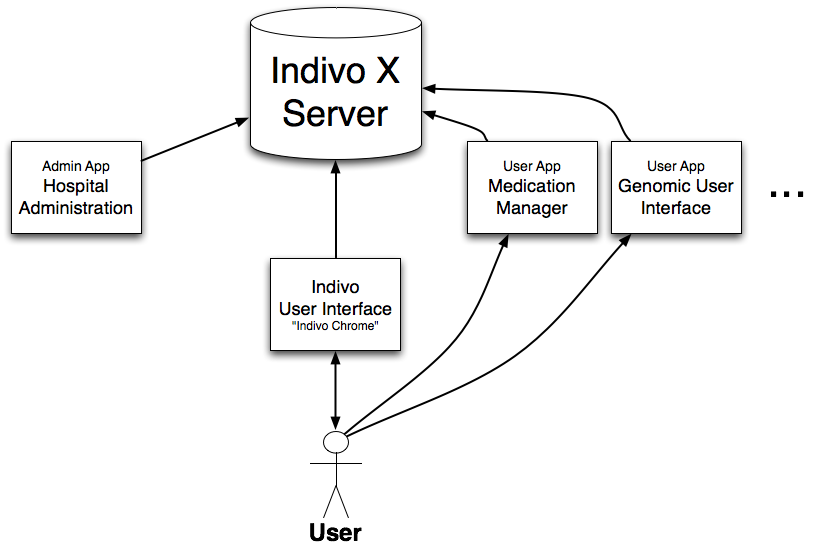
\includegraphics[width=408px,height=274px]{indivo-arch.png}
\makebox[\textwidth][c]{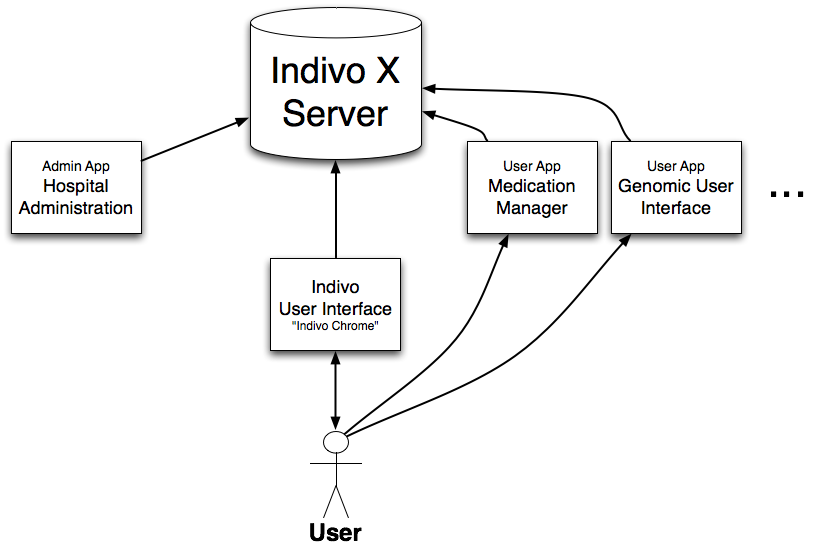
\includegraphics[width=408px,height=274px]{indivo-arch.png}}%
\caption{Indivo architecture overview.~\cite{indivoDoc}}
\label{fig:indivoArch}
\end{figure} 

A record in Indivo consists of a single or multiple documents and can be accessed by one or multiple accounts. Nevertheless there is one account defined as the owner of the record. There are different data models based on Django`s object-relational mapping (ORM)~\cite{django}. A query API\textsuperscript{\ref{API}} and a reporting API make these data models queryable. Indivo provides a SDMX\footnote{Wikipedia: Statistical Data and Metadata eXchange (SDMX) is an initiative to foster standards for the exchange of statistical information.} schema to define the format of incoming data in their SDMX specification language. The more XSD schemas (schema for XML) are used for XML validation. The pipeline for incoming data is illustrated in figure \ref{fig:indivoPipeline}. As mentioned before this data has to be in XML format and has to agree to a XSD schema. Then it is transformed according to a transform output format and converted into one or more fact objects for storage. Via the reporting API one can then query the database for matching facts. These facts will be serialized to XML or JSON for the app to retrieve.

% Figure 2.2
\begin{figure}[ht]
%\centering
%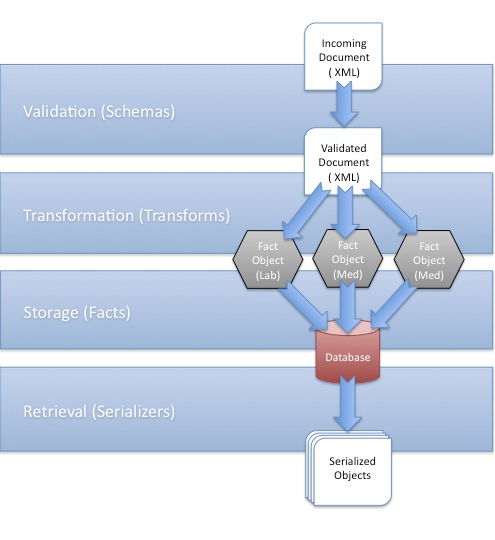
\includegraphics[width=330px,height=360px]{indivo-data-pipeline.png}
\makebox[\textwidth][c]{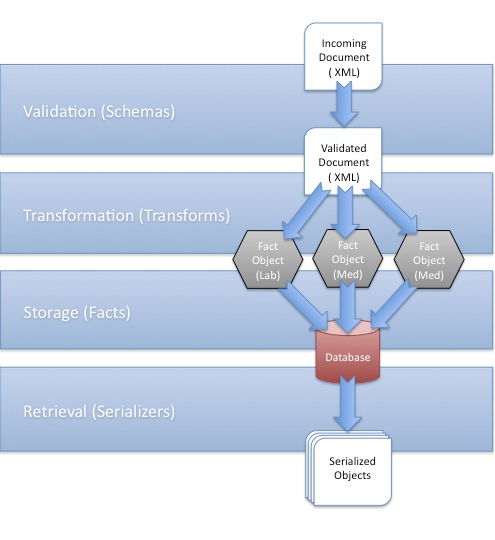
\includegraphics[width=330px,height=360px]{indivo-data-pipeline.png}}%
\caption{The Indivo data pipeline visualized.~\cite{indivoDoc}}
\label{fig:indivoPipeline}
\end{figure} 

A fact is a single data point, e.g. one medication, formatted according to a data model (here e.g. the medication data model). Indivo provides a messaging and notification system similar to emails. Messages have a subject and a body. They can be sent to records as well where they will be rerouted to the owner and all accounts that have full access to that record. To register an application with Indivo, an application manifest is needed. The SMART Project`s syntax is used for this with some Indivo-specific parameters. In the manifest the application can define among others the Indivo version to use, whether it can be used in an iframe or not, if it has an UI and the OAuth callback URL. The more there are the usual information such as name, description, version, icon, etc. The Indivo project contains many interesting ideas and approaches which we used as a starting point for our discussion on the architecture of Healthbank. In contrast to Indivo we decided not to use schemas and force others to our way of dealing with record entries. This allows to store any kind of structured and unstructured data and needs less integration work for application providers. On the contrary, this leads to less control by us. Asking queries on the data set gets more difficult. On the other hand we do not give applications that much control. E.g. an admin application in Indivo can create new accounts and change ownership of records. All applications are allowed to do on the Healthbank system is adding new entries to a user and illustrate them. So applications will not interfere with our goal of giving the users full control of their health data.

There are other interesting platforms on the web such as e.g. 23andMe~\cite{23andme}, which provides rapid genetic testing and a lot of information about a user`s DNA. On PatientsLikeMe~\cite{plm}\label{patientslikeme} patients with similar diseases can interact and share experiences with each other. From these two platforms we can learn that it is very important for users to get information and to get into contact with people who suffer from similar diseases. Therefore Healthbank shall introduce a health knowledge platform that allows users to quickly find information about diseases and medications. With the help of a clever search engine the doctors and individual people shall also be able to search for similar patients.

%%% ------------- SECTION -------------
\section{Social Platforms}
According to the Oxford Dictionaries a social network is 
\begin{quote}
"a network of social interactions and personal relationships"
\end{quote}
Therefore Healthbank will, to a certain extent, be a social network as well. Its focus is clearly to have a centralized form of storing the user`s health data. But the system will also allow to share data with doctors, hospitals as well as with friends and family. . Furthermore it allows to communicate via a messaging system and has the ability to integrate external applications. Because of these facts, we will now have a look at two of the biggest among the variety of social networks that exist today, which are Facebook~\cite{facebook} and Google+~\cite{googlePlus}.

The Google+ Wikipedia entry tells us that it was launched by the Google Inc. in 2011. By now it has more than 500 million registered users out of which about half of them are active users (they log in at least once a month). With Google+, Google integrated several services such as their image organizer and sharing service Picasa or their messaging service Google Talk (which is now replaced by Hangouts). Also it integrates rather well with other Google services such as YouTube, Gmail, Calendar or Drive.\newline 
The part we are mainly interested is the way Google+ deals with connections between users. Google+ organizes other people related to the current user in so called \emph{circles}. A user can add other users to one or multiple of his circles. A circle is somewhat like a group for sharing. Every post, photo, event, etc. can be shared with these circles. This way the user has a very fine-grained control over sharing. In contrast to other social networks, who usually operate with a one-to-one friend relation, these circle relations are only one-directional. In other words user $A$ can have user $B$ in one of his circles, but $B$ does not need to have $A$ in any of his circles. This fact is used e.g. with the so called 'Following' circle which allows users - similar to Twitter - to follow other people they do not know, but whose posts they find interesting (e.g. celebrities). We do like this circle management and took it as a starting point for our prototype user management and sharing system.

Facebook is the world`s biggest social network founded by Mark Zuckerberg in 2004. Today it has more than a billion users around the globe. More than 600 million users access Facebook via a mobile device (Source: Wikipedia). Users have their own profile and can share posts, photos, videos or links with their friends. Others can comment and \emph{like} (an appreciation of content) these items. Users can interact with each other via a messaging as well as a chat system. Connections between users are bidirectional this means that for two users to be friends, both have to agree. \newline
With the Facebook App-Centre users get a variety of games, quizzes and other applications. These games and applications are either directly integrated in the Facebook look and feel or use the Facebook API to log into and get data from Facebook (e.g. developers can use Facebook for their page user management). These games allowed companies like Zynga to make a real fortune. Applications are allowed to add new posts to the user`s chronicle in the name of the user such as e.g. sharing a new high score in a game. We are particularly interested in the application integration since we plan to allow third-party providers to write applications for Healthbank as well. \newline
With their new Graph Search, Facebook is currently deploying, they allow to ask full text queries such as "people who like to mountain bike and live in my hometown" or "towns my family visited". We are planning to have a similar kind of search engine for researchers and doctors in order to answer questions like "people with high blood pressure living in Washington DC" or "people with similar symptoms like me".
\chapter{Health Bank System} 
\label{chap:generaldesign}
 

%%% ------------- SECTION -------------
\section{Introduction} 

The Healthbank platform shall be a system where the users can administer their health data. Thereby the focus relies completely on these users. Every user is the owner of its data. 
The user controls which applications are allowed to generate data and add entries to its account. The user determines with which doctors, family members and friends record entries are shared with.
Data is generated from different sources and can be illustrated in many different ways. Applications are data sources who provide key-value data plus a tiny bit of metadata for the record entries.

The goal of Healthbank is to build a large database of information related to any kind of health aspects, e.g. diseases, symptoms, drugs, treatment methods, sports activities etc. Once the system is accepted and trusted in by the users, a search engine shall help the users, medical providers and researchers to ask complex queries.  

In the following we will give the reader an overview of the basic functionalities which we think are essential for the system. Then we go into detail and describe how we imagine the architecture and structure of data for Healthbank. Furthermore we describe the technology which shall be used for both client and server side to implement the platform. Finally we will introduce a selected amount of use cases, which define the minimum requirements for the system. \newline

The following list contains the core functionalities which are essential to the desired health system. All additional functionalities may build upon these core functionalities. The word \emph{institute} is used in the following to refer to a group of health care providers such as doctors, doctor`s offices, hospitals, dentists, physiotherapists, psychologists, special clinics and so on. 

\begin{itemize}
	\item Users can create an account and log in and log out of the system. This feature allows users to quickly find and identify their data in the system and protect it from other eyes. 
	\item Users can store, edit and delete their personal health record entries via their system account. This allows full control of a person`s own copy of their health record anytime and anywhere. 
	\item Institutes can create an account and log in and out of the system. In their account they can provide a detailed description about their area of expertise, business hours and whatever they feel useful for the users to know. This helps institutes to be seen by user and for private advertisement. 
	\item A permission system allows users to make their health record or parts of it visible to other users and/or to institutes. With this feature family, friends and institutes can inspect record entries of the user.
	\item Provided the user granted access, institutes can inspect and create new record entries in the health record of a user. This allows e.g. a doctor to upload all the relevant information about the latest visit to the user`s account or gives a hospital insight into important information after an accident happened. 
	\item An entry in the user health record shall be able to contain files (or pointers to) such as x-rays, MRI etc. next to all kind of attributes and text.
	\item A search engine allows to search for users, institutes, record entries, applications and other data stored in the system. This functionality helps to navigate in the system and e.g. to find the right institute in case of specific health problems.
	\item An API provides access to all the core functionalities as well as to possible extensions to the core. This functionality allows the system to grow and external partners to integrate and be part of the system. 
\end{itemize}  

Obviously there are many more featured a system like this could and should provide. As they all build to a certain extent on top of these core functionalities, they are not part of this list. Some of them will be discussed in the remainder of this document.
 

%%% ------------- SECTION -------------
\section{Architecture} 

In this section we describe different constructs in the overall architecture, which we think are essential for a system like Healthbank. Then we will give an overview of how we imagine the general architecture of the system and its components. At the end we will briefly talk about what kind of technologies we expect to be best suited for the architecture.

\subsection{Record Entry}

A record entry is any single piece of data entered into Healthbank. Each entry shall be assigned to and owned by a single user. Examples for entries include results of blood tests, intake of medication, running statistics, what the user ate for lunch, an ECG, a doctor`s visit etc. An entry shall be created via applications in different ways. This includes entering data manually via an application on the Healthbank web site, sending data in through email, creating data by an app on a mobile device or a gadget (e.g. smart running watch) or by bulk loading from an existing database. Entries shall have very few required metadata and otherwise contain all kind of different key-value pairs. Applications shall provide metadata to improve the search experience and to provide information on how to interpret the entry. Entries shall be displayed in many different ways by visualizations.

\subsection{Access Categories} 

The Healthbank access categories shall be very similar to the circles scheme used by Google+ (see chapter \ref{chap:relatedwork}). They shall be the main tool for the management of relations among users and sharing of record entries with others. 
Access categories shall belong to and be maintained by a single user. The user will be able to add other users, patients and/or health care providers to them. Furthermore users shall assign record entries to these categories. All entries which a user assigned to an access category are then visible by all the users in this category. In contrast to social platforms such as Facebook, our access categories are not bidirectional. User $A$ can share data with user $B$ but $B$ does not have to share
anything with $A$. This makes particularly sense if we think about a patient to doctor relation. A patient most certainly wants to share its health record data with its doctor, but a doctor has probably no data entry to share with the patient.

Our system shall be very fine-grained. The user shall be able to decide for every record entry individually, what access categories it is assigned to. The more it shall be possible to share entire folders as well as all data coming from a certain application with an access category. Initially there shall be four predefined, basic categories for family, friends as well as medical and wellness professionals. Since we are dealing with very sensitive data, there is no such thing as a public access category. But there will be a special category called \emph{science}. If a user specifies that an entry is shared with the \emph{science} category, then the user agrees that the entry may be used by scientists (without actually defining who a scientist is) for research purposes.

The system shall allow to create, rename and delete categories. Adding new users to and removing them again from categories as well as assigning categories to entries shall be straight forward. To guarantee this, the developers shall pay special attention to usability aspects for dealing with access categories during the implementation of the system.

\subsection{Folders} 

Some record entries are highly related to each other, e.g. jogging entries or different entries that result from a surgery. Therefore the Healthbank system shall provide folders to help users organize their entries. Similar to a folder in the file system of an operating system, a folder shall contain a set of entries. Folders shall belong to one user and are not visible by others. Similar to access categories it is the user`s responsibility to assign record entries to folders. The assignment to a folder shall either be done fine-grained and individually for every single entry or automatically by assigning folders to applications. In the latter case every new entry by this application will be assigned to the selected folder. \newline
Folders shall not be limited to record entries of one user only. The system will rather allow the users to add data of other users, who shared data with them, as well.

Furthermore, folders shall not only be a set of consolidated record entries but serve as the main way to visualize the information stored in the entries. Therefore folders shall contain visualizations. These will get the entries in the folder as input and are able to illustrate the information in a creative way. 

There shall be three predefined spaces. The \emph{all} space contains the most basic visualization, a simple list, and serves as a feed, much like Twitter or similar networks. This feed lists all the health record entries, events, etc. associated to the user. The other two predefined folders shall be \emph{medical} (contains all the health related information) and \emph{wellness} (contains all the fitness and wellness information). 


\subsection{Market Place} 

One important aspect of the Healthbank system will be to make it extensible and open for third-party providers. These providers shall be able to write applications which allow our users to import data to their record, either manually or from their accounts on the provider`s servers. The more these third-party providers shall be allowed to create applications that visualize the data in the user`s record. Visualizations or illustrations include graphics, statistics and side by side comparisons between users (e.g. jogging data). In order for the users to get to know such applications Healthbank shall provide a market place similar to the application centre on Facebook or the Android Play Store. 

In the following, we define the two types of applications we shall provide with Healthbank. Applications for data generation and import as well as visualizations for data illustration. 

\subsubsection{Applications}

Applications are the main data source for record entries. They shall be small pieces of code that integrate into the GUI and allow the users to add data entries to their health record. The GUI part of an application shall thereby be one of two things. The application can provide a sophisticated GUI or a form where the user can enter data manually. On the other hand, if external providers prefer business to business connections, they can provide a login form or similar. This way we allow the application to identify the user and get the required information.  \newline
Applications shall be listed in the market place where the user will browse through them and click on the desired one. In a detail view the system shall then present the user a description of the application as well as other useful information about it. A review and rating system shall help the users to identify very good applications and give the application providers valuable feedback. This review feature is not essential for a prototype but should be present in an online version of the system. 
From the detail view the user shall be able to install the applications to its account. This will automatically allow the application to get certain user data such as the name, icon and the user identification. This data is needed to make business to business communication possible. 

To illustrate the application concept we present two examples. In a medication application the user can manually add new drugs he or she bought together with time and date, prescription, the drugstore, price etc. To use this 
application the user has to be logged into the system and needs to open the application via the navigation on the page. In the GUI of the application the user can enter the data into a form and save the new entry to its health record. \newline
In a second example a company like Runtastic~\cite{runtastic} (Jogging data) cooperates with Healthbank and provides a simple application. When the user installs this application he or she has to provide the user name and password for their Runtastic account. This data is then transmitted via the application to the Runtastic servers. Now each time the user records a jogging session via Runtastic, their servers will be able to automatically call our API and add a new entry to the user`s health record. This is possible without the need of the user to be logged in. For this business to business communication the security standards shall be especially high.


\subsubsection{Visualizations}

Visualizations are responsible for illustrating data generated by applications. Similar to applications they consist of small pieces of code provided by third-party providers that integrate seamlessly into the folder structure. In contrast to applications they shall not be allowed to add any data to a user`s health record. When loaded in the folder construct the visualization will get the set of record entries assigned to this folder. Using this data they may draw graphs, create statistics, compare different users or visualize the data in any other creative way. Visualizations shall be accessible via the market place. Users shall be able to read a detailed description, to write reviews and to in- and uninstall visualizations to/from their Healthbank account. Furthermore they shall assign them to one or multiple folders. The folder to visualization relation is $n$ to $n$.

As an example one could imagine that Runtastic, after they have built their application for Healthbank, wants to show the user their effort of the last jogging sessions. Hence, they create a visualization and upload it into the market. The user installs the Runtastic visualization and assign it to its jogging folder. When the user now navigates to this folder, the visualization gets the record entries assigned to this folder. It filters out the entries generated by the Runtastic application and shows e.g. a map of the last route, a graph with speed and altitude values and statistics of the user`s overall performance. The more it allows to compare the results with friends of the current user by providing a side by side view of the statistics or by drawing an additional line in the line chart. Obviously this works only with friends who have actively shared their Runtastic data with the user.


\subsection{Health Information Platform}\label{HIP}

Additionally to the user related data the Healthbank system shall implement an information platform. This platform will assemble knowledge about different kind of health data such as e.g. remarks about diseases, medications, nutrition advices or the latest research findings. The platform can have e.g. the form of a wiki. Content shall be provided and edited by doctors and researchers or managed by the Healthbank organization itself. An essential part of the platform must be a drug register (inclusive generic drugs). It is very important on such a platform that the health facts are correct and written in an emotionless way. People tend to be very scared about diseases, so if they search for diseases using their symptoms, the facts should help to acquire knowledge and not increase the hypochondria. As PatientsLikeMe\ref{patientslikeme} and similar platforms showed, that patients like to communicate with people who suffer from the same diseases. Therefore a forum like system or a clever comment system within the wiki needs to be built to give people a platform to discuss their problems and to help each other. A well maintained knowledge database will help to build a certain trust level between the users and Healthbank and motivate the users to visit the site more frequently.
 
Other ideas we had for this platform include a doctors, hospitals and pharmacies register which helps patient to find the specialist closest to them. In this register users can review and comment on the different medical treatments they received. This way users get supported in finding the best doctor for their upcoming surgery and the health providers get feedback on what they do well and where they can still improve.


\subsection{General Architecture}

The general architecture we recommend for the Healthbank system is illustrated in figure \ref{fig:architecture}. The user communicates with the client provided by Healthbank either on a desktop web client or via a mobile version. This client then talks to the Healthbank server REST API, where the data is gathered from the database and sent back to the GUI. For the prototype we only expect to provide a desktop web version for the GUI. A second way to communicate to our server is via an external provider. This way a business to business transmission from the provider`s server to our server`s REST API will add new record entries to the user`s health record. 

% Figure 3.1
\begin{figure}[ht]
%\centering
%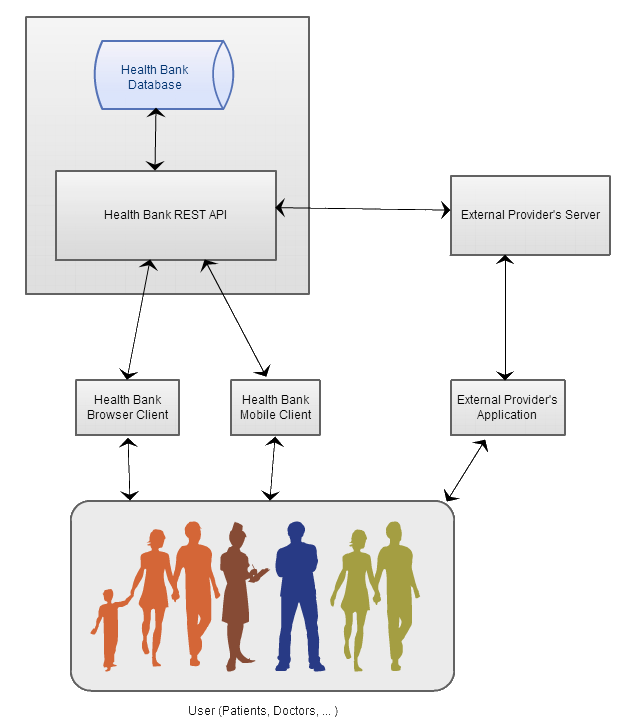
\includegraphics[width=322px,height=363px]{architecture.png}
\makebox[\textwidth][c]{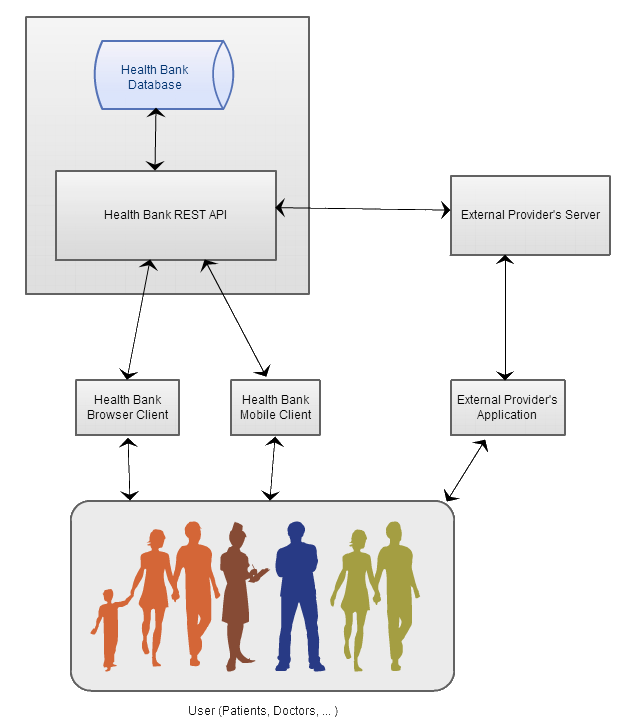
\includegraphics[width=322px,height=363px]{architecture.png}}%
\caption{General architecture of Healthbank system.}
\label{fig:architecture}
\end{figure} 

Figure \ref{fig:ERdiagram} shows an ER diagram of the basic data structure we expect the system to have. This includes the user and institute profiles, record entries and access categories as well as the interaction between them. The diagram shows in particular that it is the user who has control. The user shall create its records and assigns them in a fine-grained way to its access categories. Institutes are very similar to users, they shall create their own records or create record entries for connected users. Institutes shall also create their own access categories for sharing profile information etc. but they will have no way of influencing the user`s access categories. Access categories are always bound to a single user and no one else can view or control them. For the sake of convenience this diagram omits the fact that record entries are effectively generated by applications and inspecting entries is realised via visualizations.
 
% Figure 3.2
\begin{figure}[ht]
%\centering
%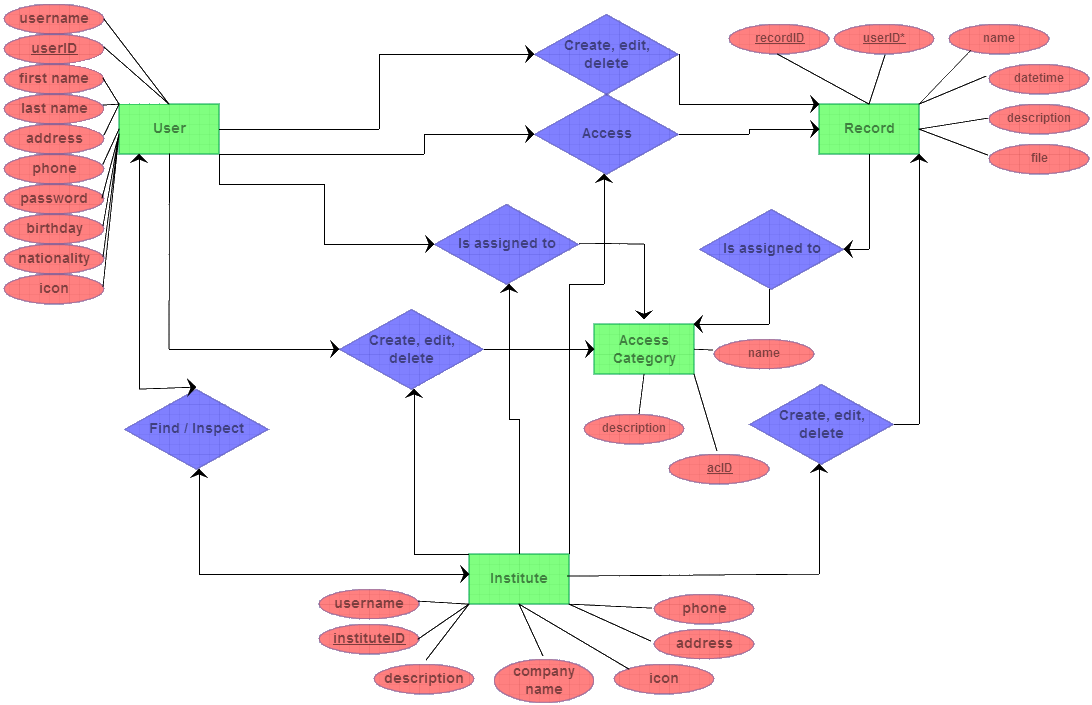
\includegraphics[width=491px,height=317px]{erDiagram.png}
\makebox[\textwidth][c]{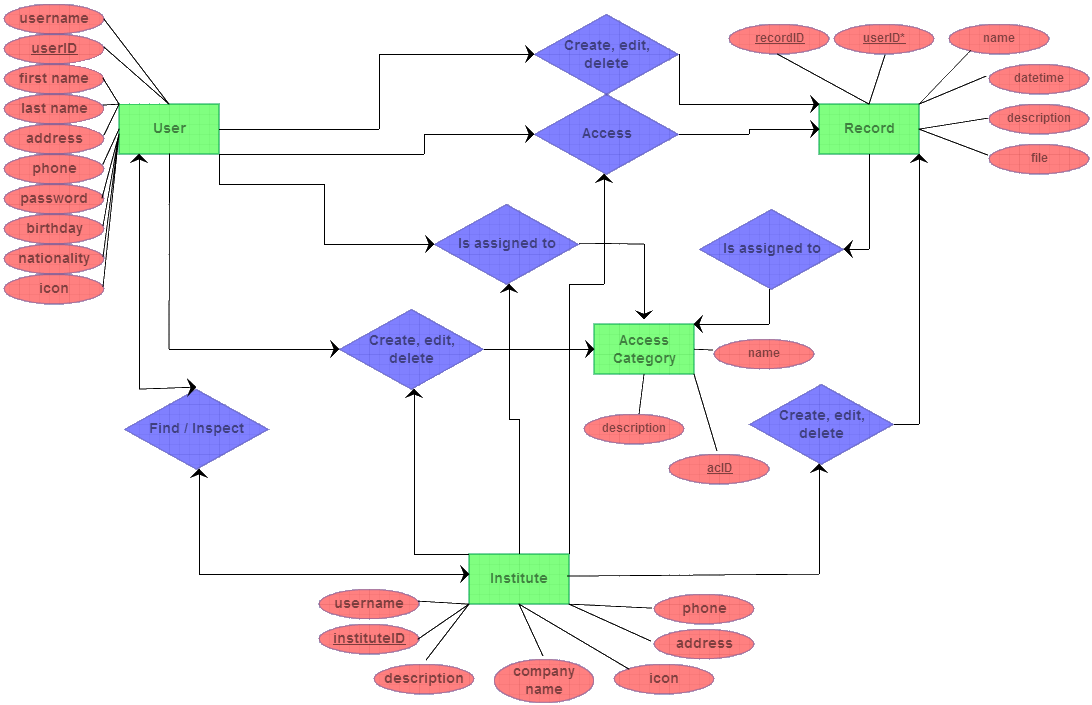
\includegraphics[width=317px,height=317px]{erDiagram.png}}%
\caption{ER diagram of the general setup.}
\label{fig:ERdiagram}
\end{figure} 


\subsection{Technologies} 

The technologies to be used for a system like Healthbank can be very different depending on the knowledge, preferences and expertise of the developers who work on the project. Nevertheless, in the following subsections we shall provide the basic requirements these technologies need to provide to be of use for the Healthbank system. 


\subsubsection{Database} 

The database needs to deal with structured and unstructured data. Apart from the rather structured data of the user accounts, applications, messages etc. the database needs to deal with different kind of record entries. These entries consist of key-value pairs with unpredictable and varying keys. They can be loaded from a SQL database, from a XML or JSON data structure, from an HTML form or even from entire files. To deal with this kind of data we suggest to use a NoSQL database which does not need detailed schema and fixed tables. Because of the JSON data structure, which should work well with a REST API and a JavaScript client, MongoDB would be a reasonable solution. Other possibilities include CouchDB from Apache, eXist, Berkeley DB, or similar databases. 
 
\subsubsection{Server}

The server shall implement a REST API which provides at least functionalities for the user to get access to its data, to store new data and to get into contact with other users. The server needs to connect seamlessly to the database and query it. There are many different approaches which would work perfectly well such as e.g. Java Servlets, PHP, Ruby, ASP.NET or anything alike. 


\subsubsection{Client}

The client is the gate to the user. It shall be user friendly and self-explanatory. If a new user creates an account it shall be very easy and straight forward to get to know the system, install new applications, find friends and upload data. Therefore the client shall be either a website with well-known patterns or a native application for a smartphone or tablet. Also a rich desktop application is conceivable. Regarding technologies the engineers implementing a client shall focus on user friendliness and a modern UI which supports animations, drag-and-drop interaction as well as touch input. For the prototype we expect it to have a desktop web application preferably built in HTML 5 and any kind of JavaScript framework.

 

%%% ------------- SECTION -------------
\section{Use Cases} 
\label{usecase}

The following table \ref{tab:usecaseTable} shows a subset of the use cases we derived for the Healthbank system. The document which contains all of the about fifty use cases is provided with the source code of the prototype. All the use cases with an id of $1.x$ in this document are applicable for both normal users and institute users. Whereas the use cases with an id of $2.x$ are only applicable for institute
users. In the table the shortcut \emph{app} stands for applications, \emph{HR} for health record and \emph{AC} for access category.
\newpage

\begin{table}[ht]
  \centering
	\begin{tabular}{c l l}
	Id & Use Case & Description \\
	\hline
	\\
	1.1 & Register user & Create and register a new user to the system. \\ 
	1.2 & Login user &  A registered user can log into the system.\\
	1.3 & Logout user &  A logged in user can log out of the system.\\
	1.4 & Add entry to HR & A user can manually add entries to its HR. \\
	1.5 & View HR & A user can view all the entries in its HR. \\
	1.6 & Edit entry in HR & A user can change the data in an entry of its HR. \\
	1.7 & Delete entry in HR & A user can delete an entry in its HR. \\
	1.8 & Change personal settings & A user can change its profile settings. \\
	1.9 & Search & A user can search entries, other users and apps. \\
	1.10 & View record of other user & A user can view shared entries of another user.  \\
	1.11 & Create AC & A user can create AC to control data sharing. \\
	1.12 & Add person to AC & Users can add other users to its ACs to share  \\
	 & & data with them. \\
	1.13 & Remove person from AC & Users can remove other users from ACs. \\
	1.14 & Change entries AC assignment & Users can for each entry change its assignment  \\
	 & & to ACs. \\
	1.15 & Edit AC & The metadata of an AC can be changed. \\
	1.16 & Delete AC & An AC can be deleted. \\
	1.17 & Group entries into folders & Multiple entries can be assigned to folders for  \\
	 & & a better overview. \\
	1.18 & Install app to profile & Users shall be able to install external apps  \\
	 & & from a market. \\
	1.19 & Remove app from profile & Users shall be able to uninstall installed apps. \\
	1.20 & Send message to other user & Users can send messages to other users. \\
	1.21 & Delete profile & Users shall be able to remove their profile from  \\
	 & & the system \\
	\hline
	\\
	2.1 & Institute adds entry to user & An institute shall be able to add entries to users,  \\
	 & & if they allow. \\
	2.2 & Institute profile different & The profile of an institute user shall be different  \\
	 & & then of a normal user. \\
	2.3 & Query engine & Selected research institutes shall be able to use  \\
	 & & a sophisticated search engine for the big data. \\
	2.4 & Add app to system & Institute users shall be able to add new apps  \\
	 & & to the system. \\
	2.5 & Edit app data & The app author shall be able to update and change  \\
	 & & app information. \\
	2.6 & Remove application & The app author shall be able to remove an app  \\
	 & & from the system. \\
	2.7 & App adds entry to user & Apps shall be able to add new entries to user`s  \\
	 & & record, if they allow. \\
	2.8 & App illustrates record & Apps shall be able to visualize a set of entries in the  \\
	 & & user record, if they allow. \\
	\end{tabular}
	\caption{A subset of the use cases for Healthbank}
  \label{tab:usecaseTable}
\end{table}
 
%%% Local Variables: 
%%% mode: latex 
%%% TeX-master: "thesis" 
%%% End:
 

\chapter{Prototype Implementation}
\label{chap:prototype}

To give a proof of concept, we implemented a prototype which shows a good selection of the functionality expected by the Healthbank system. The prototype is intended to show the possibilities of such a system as well as to build a solid basis on which future work can build upon. In the remainder of this chapter we discuss in detail the data model, architecture and technologies used for implementing the prototype.


%%% ------------- SECTION -------------

Because of the extensibility and reusability constraint on the system, we decoupled the implementation of the server and client into two completely separated projects. The server has direct access to the MongoDB~\cite{MongoDB} database via a socket connection on the localhost. The connection between client and server is done via HTTP and AJAX requests to the server REST API. In figure \ref{fig:prototypeSetup} we illustrate this relation.

% Figure 4.1
\begin{figure}[h]
%\centering
%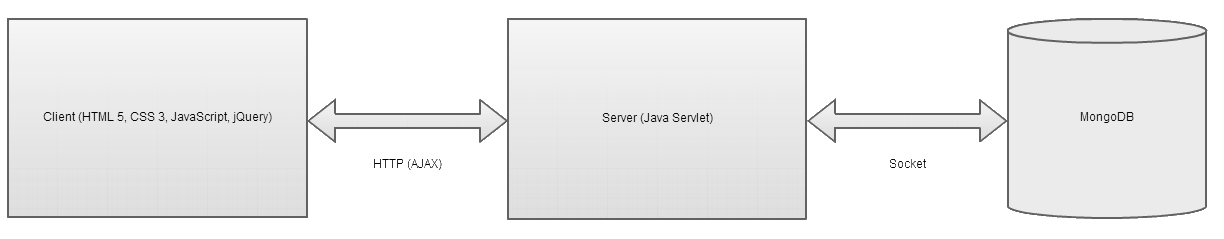
\includegraphics[width=408px,height=80px]{prototypeSetup.png}
\makebox[\textwidth][c]{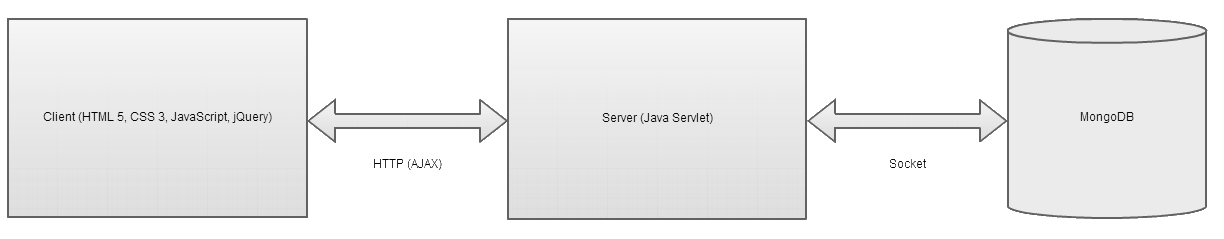
\includegraphics[width=408px,height=80px]{prototypeSetup.png}}%
\caption{Components of the prototype.}
\label{fig:prototypeSetup}
\end{figure} 


%%% ------------- SECTION -------------
\section{Data Model}

As supposed, we used an instance of MongoDB~\cite{MongoDB}, which is open-source, agile, scalable and one of the leading NoSQL databases at the moment. The JSON-style~\cite{JSON}, document-oriented storage works very well for our purposes, since we can use JSON as the main communication format for our AJAX calls between server and client. \newline
The following table \ref{tab:collectionTable} describes all the collections (equivalent of an RDBMS table) used in the MongoDB instance to support our functionalities:\newline

\begin{table}[h]
  \centering
	\begin{tabular}{l l}
	Collection name & Description \\
	\hline
	applications & Contains application specific information. \\
	 & Icons are saved in applications.files collection.\\
	circles & Contains all information about user`s circles \\
	messages & Contains messages sent between users \\
	news & Contains news entries \\
	records & Contains all health record related data. \\
	 & Files are saved in records.files collection. \\
	spaces & Contains all information about user`s spaces \\
	users & Contains all user related data such as name, address etc. \\
	 & Icons are saved in users.files collection.\\
	\end{tabular}
	\caption{The list of collections used on the MongoDB instance}
  \label{tab:collectionTable}
\end{table}

Every entry in a collection contains an ObjectID which identifies the object uniquely within the database. The more every entry has a field called \emph{timedate} which holds the time and date of the object creation. As it is a MongoDB database, all data is saved as JSON and hence in a key-value style. Here is an example of a message collection entry representing a message sent from one user to another.\newline

\begin{lstlisting}[language=json,firstnumber=1]
{
        "_id" : ObjectId("id"),
        "message" : "This is the first ever test message. Fingers crossed...",
        "read" : "true",
        "recipientID" : "id",
        "senderID" : "id",
        "subject" : "The first message of all time",
        "timedate" : "07/11/2013 12:50:47"
}
\end{lstlisting}

The \emph{ID} fields contain the mentioned ObjectID values of the respective user. Such an ObjectID values is composed of the current time, machine id, a process id and a random value.

%%% ------------- SECTION -------------
\section{Concepts}

In this section we describe the concepts used in the prototype to implement the requirements from chapter \ref{chap:generaldesign}. 

\subsection{Login and Session Management}\label{loginSession}

Authentication and session management is generally a very tricky task. For the prototype we decided to apply a rather simplistic but solid method. This method omits cookies and builds on top of the new HTML5 storage possibilities, especially the local storage~\cite{localstorage}.

The user needs at least a unique user name and a password to register. When the login with user name and password was successful, the system will generate a session key for the user and set an expiration time for the key. The session is set to expire after one hour of inactivity. With every request to the API by the user, the session key has to be provided as well as a credentials value. These credentials are the composition of the user name and password in a hashed form for security purposes. The session key and the credentials value are stored locally on the client device and are read by every call to the REST API. If the session has expired or there was any other issue, the user is automatically passed on to the login page. 

\subsection{Circle}

The concept of circles is one of the most essential in our system. Circles are what we called access categories in chapter \ref{chap:generaldesign} and allow the user to share any record with other users such as friends and family or doctors and hospitals. The concept is in many ways similar to the one used by Google for their social media platform Google+~\cite{googlePlus}. We chose to adapt Googles concept, because we like it and we think that this way it will be easier for the user to get used to it, compared to something new and unique. \newline
There are two aspects to circles which needed to be considered in the prototype. Firstly, there is the creation and manipulation of circles as well as the assignment of other users to them. Secondly, is the assignment of record entries to circles. In the GUI these two aspects are separated but logically they are highly coupled. All the record entries assigned to a certain circle are automatically visible by users assigned to the very same circle. 

On the webpage we designed a dedicated page for the circle management (see figure \ref{fig:circlesScreenshot}). On this page the user will see four predefined circles for $Family$, $Friends$ as well as $Medical Professionals$ and $Wellness Professionals$. These four circles are fixed and the user cannot delete or change them apart from their colour. By clicking on the circle with a $+$ sign in the centre the user can add a new circle. A circle consists of a name, a description and a colour for illustration purposes. User created circles can be edited and deleted. To see the users in a circle or to edit one, the user can click on them. As a result of a click we will show a list of rectangles containing the user icons and names of the users present in the circle as illustrated in figure \ref{fig:circlesScreenshot}.  The more, next to this list there are buttons to edit and delete (only on user generated circles) the circle as well as to add spaces (see next subsection \ref{spaces}) to a circle. This last button actually allows the user to add all records who were assigned to this circle, and will be assigned to it in future, to the specified space. Spaces are the implementation of the concept of folders and will be explained in the next subsection. The rectangles in the list have drag-and-drop support which can be used to move them to the trash (remove a user) as well as to assign them to other circles (by dropping on a circle). To find users in the first place the circles page also contains a search field on top which allows to find users by user, first, last or company name as well as by email. 

% Figure 4.2
\begin{figure}[h]
%\centering
%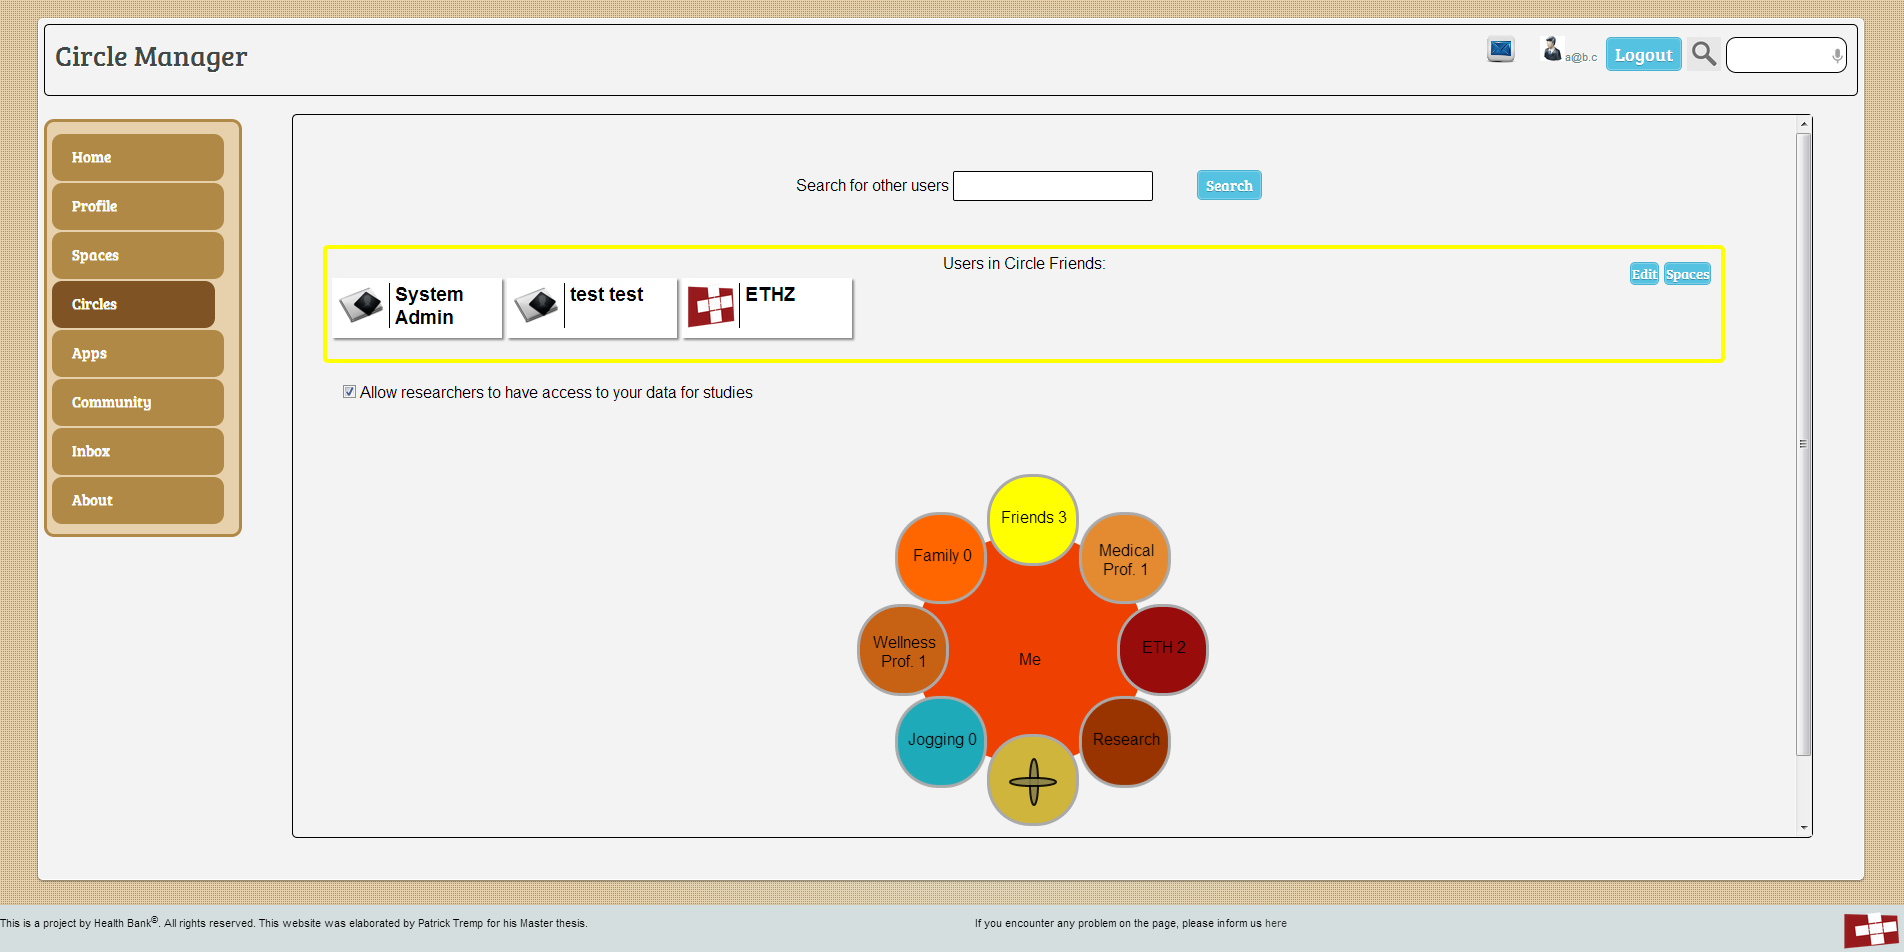
\includegraphics[width=476px,height=238px]{circlesScreen.png}
\makebox[\textwidth][c]{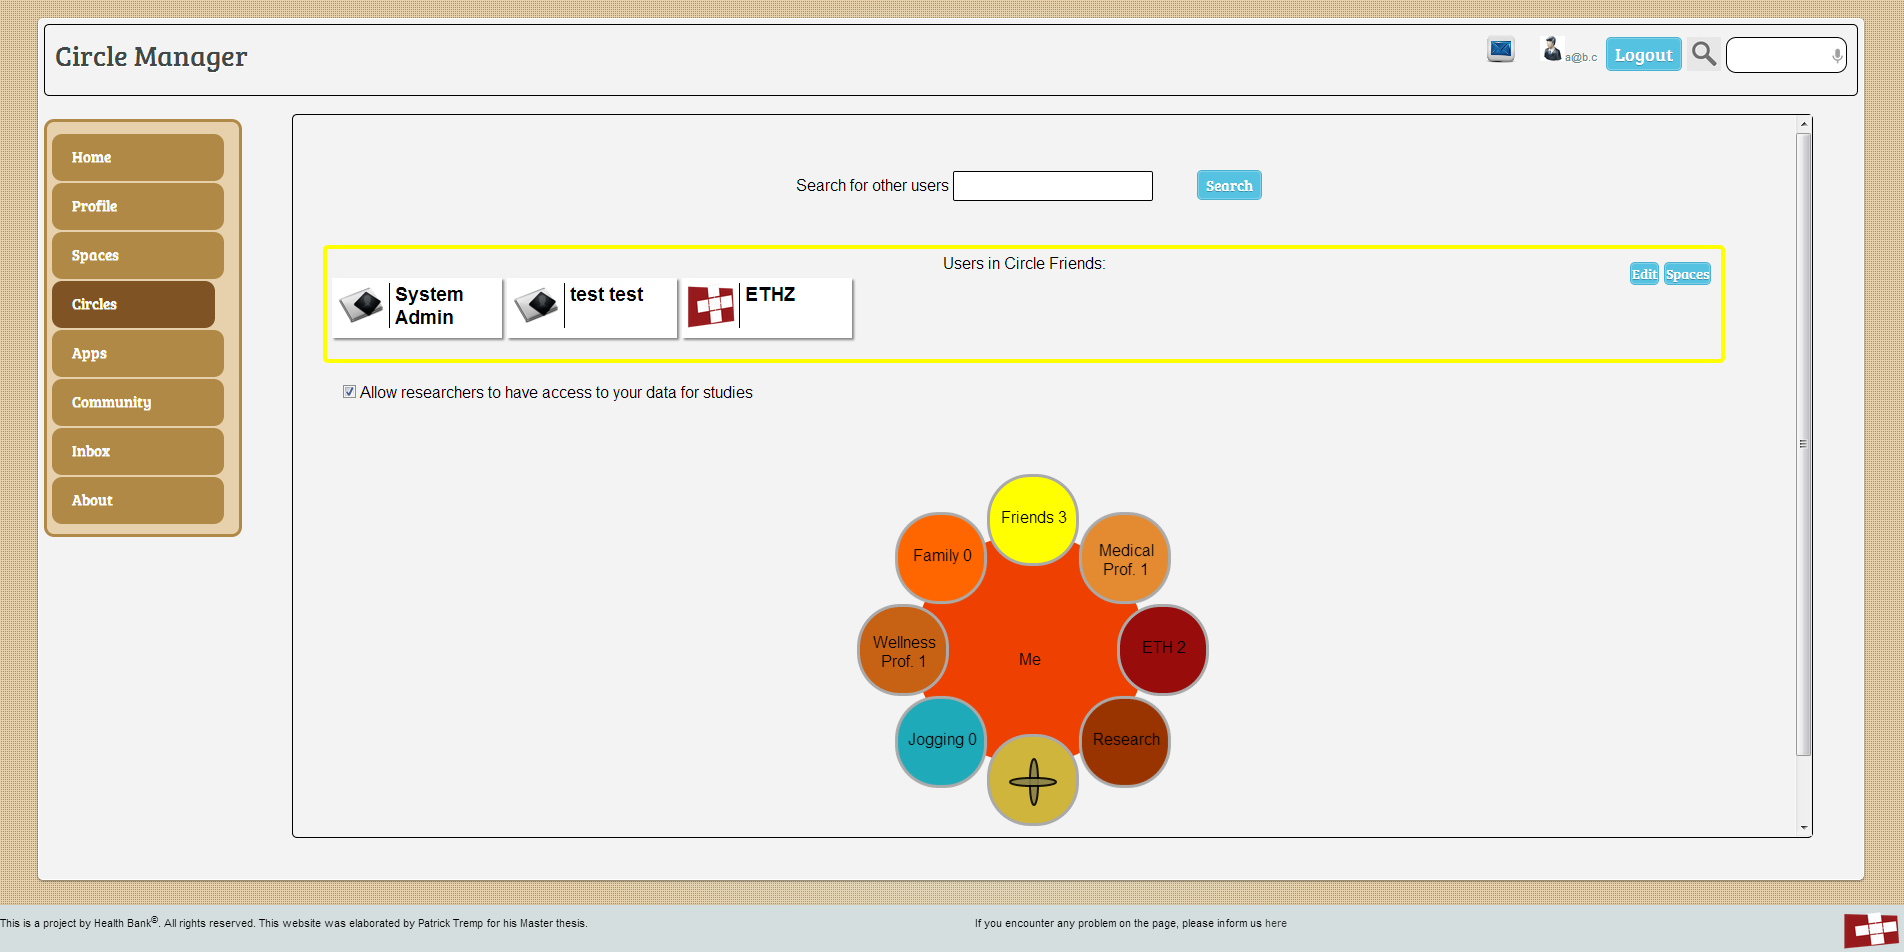
\includegraphics[width=476px,height=238px]{circlesScreen.png}}%
\caption{Screenshot of the circles page in the prototype}
\label{fig:circlesScreenshot}
\end{figure} 


\subsection{Spaces}\label{spaces}

In chapter \ref{chap:generaldesign} we defined the concept of folders. For the prototype we called this concept spaces. Generally speaking a space is a set of entries in a user`s health record. Additionally a user $A$ can also put entries from other users, who shared some entries with $A$, into its spaces. Nevertheless spaces are always bound to one user and other users are not allowed to see or change $A$`s spaces. Besides the list of record entries assigned to the space, a space can also contain a visualization. This visualization will get all the record entries in the space as input and may use them to create beautiful illustrations. 

Users control their spaces in the spaces page of the prototype. Whenever the user clicks on the spaces link in the navigation, the so called $All Space$ will be shown, which contains all the recent record entries of the user. This \emph{all} space is similar to the Twitter feed of a user or the Facebook chronicle. \newline
On top of the list there is a dropdown menu for filtering. Filtering allows the users to inspect record entries of users who shared their data with them. In this menu the user can select other user individually or even entire circles. By selecting $no filter$ all users from $A$`s circles will be selected. The selection of another user $B$ in the filter dropdown has the consequence that all the entries, which $B$ has shared with $A$, will appear on the list. By selecting an entire circle, all the entries, which the users in that circle shared with $A$, will appear on the list. Entries by other users will be indicated as such by a colouring system. It is possible that a user will not see any record entries of $B$ when $B$ is selected in the filtering menu. This can happen, when $B$ does not share anything with $A$. The filtering menu will be present in all of the different spaces. In all but the \emph{all} space there is the additional restriction, that only entries of other users will be shown, which $A$ has assigned to the particular space.

At the very top of the spaces page there are multiple tabs for navigation between the different spaces. The user can control the order in which the spaces appear in this tab list, create new spaces and edit them by clicking on the gear icon at the right hand side. A space is defined by a name and a description and can optionally contain a visualization. An additional feature allows to hide spaces, which the user currently does not use, on the tab list. This helps the users to keep the list clean and short. 


\subsection{Profile}
As described before the profile of a user has to contain at least a user name and a password. The more, we ask for the first and last name in the registration process. Once logged into the system, the user can visit the profile page any time and edit its data. Besides properties like the address, phone numbers, insurance type etc., users can also change their user icon and password. For institute users the profile page looks slightly different. Rather than detailed information about the individual user, institutes can enter a description of the company including what the company is known for, opening hours etc. Also on the profile page the users can decide to which circles they like to share its profile data. So far we have an all or nothing policy. Either the user shares all its profile data with its selected circle or only what is publicly visible. Publicly available are the user`s name as well as the user icon. This data is shown e.g. when a user searches for other users. The detail view opens when you click on a user entry. Depending on whether or not you are in one of the circles, this other user selected for profile sharing, this detail page will show only the public or all profile data. 

Technically we solved the profile sharing by storing user data twice. Usually all profile data is stored in the users collection of the database as described in the collection list above. Non critical fields, such as the users first and last name, the icon, the address, phone numbers, email etc., are then additionally stored as an entry in the users health record. This entry gets updated each time the profile is updated. By doing so we can now apply circle information to that entry and share this with other users. In other words the profile information stored in the users collection is not accessed for showing user`s details. Hence, no sensitive data such as the password, session key or similar is ever visible for other users.


\subsection{Applications}

In the prototype the user can access the application section via the navigation. Patients will be able to go to the market, where all the applications and visualizations are listed and their details can be inspected. The more, they can access a list of all the applications as well as visualizations which they have already installed to their account. Institute users on the other hand have some more possibilities. They can add new applications or visualizations, see and edit the applications and visualizations they have already contributed to the system and inspect the developer guide. 

In the prototype applications contain a name, a description and an icon. Furthermore, the author can specify a version number, define if the application is on- or offline (visible in the market or only accessible by the author) and for whom the application was built for (users, institutes or both). The applications have to be written in HTML with the help of CSS and JavaScript. To keep matters separated, the author can upload individual files for HTML, CSS and JavaScript content. Once the application is in the system the author can edit the information and populate a field called 'what is new'. With this field the author can tell the clients what has changed in comparison to the last version, similar to the Android market. When a new application is uploaded, it gets a unique identification as well as an application secret. These values are only visible for the author. The secret is needed for B2B communication and can be refreshed if needed. 

Once the user has seen the details of an application and hit the install button, the application can be accessed by clicking on them. The application code is loaded into an iframe component on the page and runs from there. As mentioned in chapter \ref{chap:generaldesign}, we provide two methods for adding new entries to the user`s record. The straight forward way is the manual insertion of the entry by the user. With this method the user enters data directly from within the application running in the iframe while the user is already logged in and has a valid session key. This information is used by the client API to access the server and add the entry to the record. The second method allows business to business communication from the third-party server directly to our server. During this process no user needs to be logged in. Therefore we needed to come up with a different authentication solution for B2B communication. The solution, we have chosen, is illustrated in figure \ref{fig:b2b}. Illustrated as $1)$ in the figure is the process of installing the application on our system. When the user installs the application and opens it on the Healthbank GUI, we expect that the application shows a login form or similar, where the user can login to the partners service (e.g. Runtastic). When the login is successful, the external service will also know the user`s identification on the Healthbank platform and may store this along the other user data. When the user creates a new entry later on in e.g. the mobile application of the third-party provider, this entry gets stored in the user account on their server (see $2)$ in the figure). Now the other server will query the stored Healthbank user identification and send this value together with the application identification and application secret to our REST API. If all the values are correct, our system will generate a one-way access token and send it back to the external service. Finally, the service can call our \emph{add entry} API providing the access token, user and application identification and the actual record entry data. More details and information about the API is available from the documentation in the developer guide of the prototype. 

% Figure 4.3
\begin{figure}[h]
\makebox[\textwidth][c]{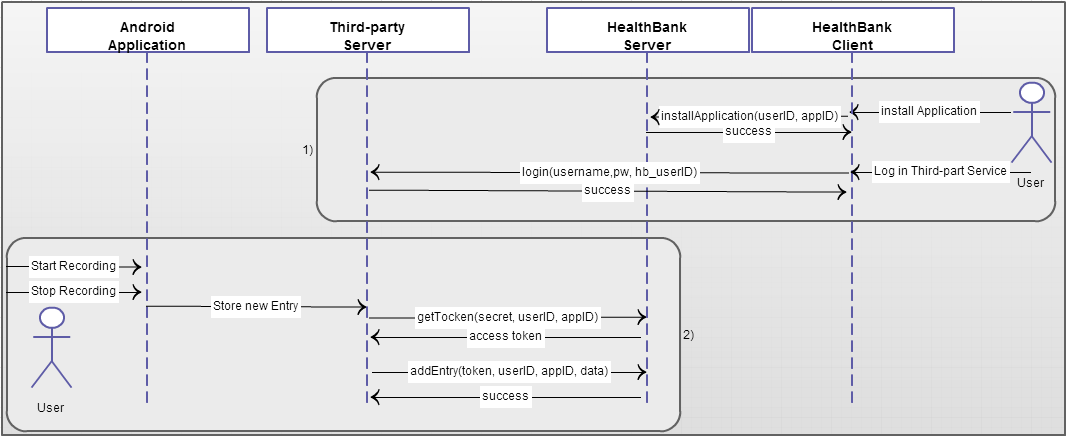
\includegraphics[width=355px,height=145px]{b2b.png}}%
\caption{Illustration of business to business communication to add new entry}
\label{fig:b2b}
\end{figure} 

As a first attempt to optimize for searching on the diverse field of data entries, we introduced index keywords. We ask the authors to provide these with the application information. Since applications have to store data in a key-value style, these index fields correspond to a set of keys which are most important to identify the record entry.

With this thesis we provide some initial applications. Most of them are rather basic and allow the user to upload simple health data via a form in the GUI. One application is particularly built for the users to add medical data. Another one is the equivalent for health care providers, which allows them to add medical data to a patient`s health record. There is an application for keeping record on the medications the users took. Two applications are part of a calories counter and allow calories intake with a food picker as well as calories burning with sports and daily calories consumption. Finally, an application is provided to keep track of endurance sports by providing the activity, duration, covered distance, heart rate etc.\newline
Following is a listing to give you an overview of how a record entry generated by for example the application to add medical data looks like on our database.

\begin{lstlisting}[language=json,firstnumber=1]
{
		"userID": "id",
		"app": "addRecord",
		"fileID": {
				"\$oid": "id"
		},
		"cause": "This is a test",
		"_id": {
				"\$oid": "id"
		},
		"timedate": "08/21/2013 14:23:47",
		"name": "File upload test",
		"fileName": "testFile.png",
		"descr": "This is a test to upload a file with a record",
		"doctor": "Dr. Test"
}
\end{lstlisting}


\subsection{Visualizations}

Visualizations are in many cases very similar to the applications defined above. They do also contain a name and a description, version number etc. Also they are defined in HTML / CSS / JavaScript files and are integrated to the GUI via an iframe. The main difference is the underlying concept. Visualizations are not allowed to add any data, but they can use the client API to access the entries of the space they are assigned to. This data can be used for drawing graphs etc. The most basic visualization, a simple list of the record entries, is present in every space page without the need of the user defining it initially. Next to this list, the user is allowed to add one visualization to each space, which will be integrated in an iframe on top of the list. When the page loads, the visualizations are able to get all the entries assigned to the particular space via a call to $parent.records$.

With the thesis we provide two initial visualizations. The first one is related to the two calories counter applications. It will search in the provided entries of the space, it is integrated to, for entries of one of the two applications. Then it uses these entries to build statistics about daily consumption and burning as well as overall data. The more it uses the Google Chart API~\cite{chartapi} to draw column charts. The second visualization is built for the endurance sports application and shows statistics about e.g. the total covered distance or duration. The more it illustrates the different attributes in graphs showing the progress over the latest entries.


\subsection{Messaging System}

The messaging system implemented for the prototype is rather basic and allows to send messages to only one other user at a time. A message contains a recipient, a header and the actual message. Users can access the messaging system either via the message icon in the action box on the very top of the screen or via the navigation link $inbox$. The message icon in the action box will change colour and begins to shake, when there are unread messages in the inbox. From the detail view of a message users can directly reply to it. Messages can be sent to any user in the system. There is no need for the users to have each other in its circles to send messages. 


\subsection{Queries}

Queries are executed only on the users and records of users that actively allowed researches to inspect their data. Therefore the query answers will not contain any data of users who did not set the research checkbox on the circles page. In the current prototype we implemented three types of search queries an institute user can use. In the following we describe these three types individually.

With a user query an institute can search for users by selecting certain constraints on e.g. the age, height, weight or the country the user lives in. In addition they can limit the search results by providing certain keywords which the record entries of the users shall contain. This query will help researches, if they search for users to participate in a certain study or similar. From the results list one can directly contact the users by the prototype`s messaging system. \newline
The second query type is used to search for certain records according to a set of keywords. This allows to search for symptoms of diseases, certain kind of injuries or similar. If there are multiple keywords separated by a space, the query performs a logical OR search on each keyword and returns record entries that contain any of the keywords.\newline
For the third type of search we used the new MongoDB text search. Since MongoDB version 2.4 they provide a text index which can be applied to all fields of a document that contain string values. Text search uses stop words, suffix stemming and is case-insensitive. With this framework we can ask queries with multiple terms (logical OR), by exact phrase searches (escape terms with quotes) and with negated terms (minus sign prefix). 

\subsection{Developer Guide}

Institutes can access the developer guide via the navigation in the apps part. The guide contains a documentation on all the services of the REST API running on the server as well as all the functions of the client-side API via JavaScript. The more we provided demos and all the information needed for creating new applications and visualizations. It has a separate design and is illustrated with code listenings and screenshots. 

\subsection{Security}

Even though security is a very important aspect for Healthbank, we did not emphasise too much on it. Nevertheless, there are a few points worth mentioning. 

We have already talked about our login and session management in chapter \ref{loginSession}. All passwords used for this process are stored encrypted in a MD5 hashed form on the database. We are aware of the fact that the MD5 hash function is severely compromised lately, but it still provides a sufficient amount of security for our purposes. The more, we never return the password hash to any client via a call to the REST API. 

We allow to upload many file types with record entries to our server. All of these files are stored directly in the MongoDB database. This is done to make sure that possible malicious files, which could harm the system, are not accessibly from outside and are never executed on the system itself. We used the GridFS specification for storing and retrieving the files in the database. GridFS was built to allow for storing files that exceed the BSON-document size limit of 16MB.

Authentication is disabled by default on MongoDB and we kept it that way for the process of implementing the system. However, MongoDB provides strong security, risk management strategies and access control~\cite{mongosecurity} which could be deployed if need be. 


%%% ------------- SECTION -------------
\section{Technologies}

In this section we describe the technologies we used to implement the different parts of the prototype. 


\subsection{Database}

As mentioned several times before, we used an instance of MongoDB~\cite{MongoDB} for our database. The MongoDB instance runs on the localhost on the same machine as the Tomcat server for the REST API. All the connections to the server run via the singleton class \verb+MongoDBConnector+ which implements our \verb+DBConnector+ interface. The interface includes queries, deletions, updates and insertions as well as methods to connect and set up the database. Because of the little data available for the prototype, we only used one server for now. Replication and sharding is documented very well on the MongoDB documentation website. Hence, it can be applied without too much effort as soon as the system is used by more users. For debugging we used the MongoDB shell tool, which allowed us to directly inspect and manipulate the database with the same queries as we used in the Java Servlets. As exemplified in the security section above, we omitted the authentication process on the locally running MongoDB instance for simplicity reasons. In the class \verb+MongoDBConnector+ of the backend the authentication is already prepared but still commented out. A description on how to apply a user name and password is present as well. All collection names, the host address and port of the database as well as the database name itself are loaded and parsed from a configuration file written in XML. 


\subsubsection{Indexes}
MongoDB defines indexes on a per collection level. Indexes can be set on single or multiple fields and are saved in a b-tree structure (see MongoDB documentation~\cite{MongoDBDoc}). Every collection has a default index on the $\_id$ field. To set our own indexes we are able to choose from a variety of options. MongoDB supports indexes on sub-documents and embedded fields as well as defining compound and multi-key indexes. We can set indexes to be unique, which guarantees, that the index field is unique, or to be sparse, where only records with this field defined will be indexed in the collection. Furthermore, there are hash as well as geospatial indexes and queries.

For our prototype we analysed the queries we ask most often and set a number of indexes to our collections to optimize for these queries. In the following list, we go through our collections and define the indexes we came up with:

\begin{itemize}
	\item Users collection: We do a lot of queries to the user name field of the user collection. Hence we set a secondary index on this field and set it to be unique, since we do not allow to set multiple user name fields. Hence in the user collection we have a total of two indexes, the standard index on the $\_id$ field and one on the user name field.
	\item Circles collection: Most of the queries to the circles collection use the $\_id$ field or the $userID$ field. Hence we set an additional index on the $userID$ field, so the database can decide, if the performance with the standard $\_id$ index is quicker than the one for the $userID$ field. Again we set the index to be unique, since obviously the userID for a circle has to be unique.
	\item Spaces collection: For the spaces the same as for circles applies. Hence we set an additional index on the $userID$ field.
	\item Messages collection: On the messages collection we set a compound index on the $senderID$ and $recipientID$ fields since this allows to optimize queries for the communication between two users. 
	\item News collection: For the news collection we did not set any additional indexes. Most of the queries use the $\_id$ field, the more the amount of news entries to expect is rather low compared to other collections.
	\item Applications collection: We set a compound index on the fields $userID$ and $appID$. This shall speed up queries to installed applications and during the (un)installing process. For requests to applications we usually use the $\_id$ field and hence, we need no additional index.
	\item Record collection: Apart from the standard $\_id$ index, we also set one to the $userID$ field since many queries use this field. Again we set it to be unique. In addition, we set a text index on all fields of the collection for the text search query defined above.
\end{itemize}


\subsection{Server}

On the server we used Java Servlets~\cite{JavaServlets} to implement the REST API and the MongoDB Java Driver~\cite{mongoJavaDriver} to get a connection to the database. There are eighteen servlets in total in the prototype so far, each defining individual functionalities accessed via HTTP GET or POST requests. The more, there is a \verb+DBConnector+ interface with an implementation for MongoDB, that handles the connection and queries to the database, as well as a \verb+CoreManager+ class, that deals with core functionalities used in multiple servlets. File manipulation and hashing for security aspects was done with the help of libraries from the Apache Commons project~\cite{apachecommons}. For parsing JSON data we used the JSON.simple framework~\cite{jsonsimple}. During the implementation we worked with Eclipse and deployed the servlets on a Tomcat server version 7.0 on Windows 7. For testing purposes and to make it publicly available we deployed the WAR file on a Tomcat server running on an ETH Debian server.

\subsection{GUI for Client}

The client is completely decoupled from the server side and runs on any kind of HTTP server such as an Apache or Tomcat server. It consists of a number of HTML, CSS and JavaScript files. Common components such as the navigation or the action box on the top right of the screen are loaded dynamically from a common source. When we change these components this brings the advantage of less copy and paste for the individual files. For Document Object Model (DOM) manipulation and other useful features we used the JavaScript library jQuery~\cite{jQuery} and the jQuery UI plugin. 
\newline
For every page we use a single HTML file. Since the GUI has become rather big over time, we favour this solution in contrast to a single page architecture, such as solution built with the Google Web Toolkit~\cite{gwt} or similar. All these pages share the $healthbank.js$ JavaScript file and $healthbank.css$ cascade style sheet. We tried to put all the JavaScript code into a single file to reduce the overall amount of files to be loaded by each request. When the DOM of any page is loaded we first call the $initialize()$ JavaScript function. This function includes loading the correct navigation and action box, querying user profile data, checking for new messages and the like. Then we load the actual content for the page. Whenever appropriate, we added some animations and transitions using the new CSS capabilities. This shall give the page a more modern view and interactions the users are familiar to. Dialogs and pop-up menus are often loaded dynamically, so we can reuse as many of them as possible (e.g. menu for adding circles and spaces). \newline
For the developer guide, which serves as the documentation for the prototype, we used a different design then on all the other pages. Navigation is still on the left but there is no action box and user related content. This design is rather simplistic and static and is loosely based on automatically generated Java Doc HTML pages.

\textbf{Communication} \newline
The communication with the server was done using AJAX (Asynchronous JavaScript and XML) requests who call the server REST API. Apart from the login, which is dealt with separately, all of these AJAX request are defined in the $healthbank.js$ JavaScript file. The REST API so far only supports GET and POST requests. With the help of jQuery the requests are rather straight forward and contain the data to send, the type (POST, GET), the URL and the data type to deal with. The response is mostly provided in a JSON structure. Most of the responses provide, next to the data, information about, if the session is still active and if the call was successful or not. In case of a success the \emph{values} field contains the desired data (e.g. an array of record entries), in case of an error the \emph{error} field contains the error message. When the session key is expired or the credentials are wrong, the functions will automatically redirect the user to the login page and no data is returned. In the following listening we illustrate a successful followed by a failed request to the user query.

\begin{lstlisting}[language=json,firstnumber=1]
{
    "result": "success",
    "loggedOut": "false",
    "message": "Here are the results.",
    "values": {
        "users": [
            {
                "userId": {
                    "$oid": "id"
                },
                "userIcon": {
                    "$oid": "id"
                },
                "lastname": "Tremp",
                "firstname": "Patrick"
            }
        ]
    }
}
{
    "result": "failed",
    "loggedOut": "true",
    "error": "Either your session timed out or you forgot to send me the session and credentials."
}
\end{lstlisting}



%%% Local Variables:
%%% mode: latex
%%% TeX-master: "thesis"
%%% End:
\chapter{Evaluation and Analysis}
\label{chap:evaluation}

After having implemented the prototype, we evaluated it by taking into account our initial design and use cases. In the next two sections we discuss, how well the prototype already fits to our use cases and how the design guidelines from chapter \ref{chap:generaldesign} were implemented. 


%%% ------------- SECTION -------------
\section{Use Case Analysis}

In this section we will discuss what use cases from chapter \ref{usecase} the prototype has implemented and what is still missing. The more, we will discuss how the user can access the described functionality as well as some benefits and drawbacks of the implementation. For the remainder of this section we describe the current and active user as $A$ and any other user $A$ deals with as $B$.

When $A$ opens our website the login screen will appear. There $A$ can enter its user name and password to log into the system. This view also allows to register a new user via a click on the register button. Once logged in, there is a logout button in the action box on the top right of every page of the website. Hence use cases $1.1$, $1.2$ and $1.3$ for registration, login and logout are implemented as required. 
\newline
Use case $1.4$ is described further down. To view the health record as use case $1.5$ demands we introduced the concept of spaces, as described in chapter \ref{chap:prototype}. Once $A$ clicks on the spaces link in the navigation the \emph{all} space appears, where all the latest entries are shown in a list view similar to a Twitter feed. \newline
$1.6$ and $1.7$ ask for editing and deletion of entries. This functionality has only been implemented on the server side for the prototype yet. There is no GUI component which uses this functionality. The user can only edit the circle and space assignments for the individual entries. The reason for this is that there are still too many open questions which need to be resolved with the stakeholders. Editing becomes a problem if the data is not generated by the users themselves. It would be rather critical if the user could change the findings of its doctor, a drug prescription or data from an application (e.g. calories burned while jogging). Deleting is a problem on all social networks nowadays. Some of them just do not show the item to the user anymore but do not actually delete the entry for years. For our platform we would of course prefer, if entries would be kept anonymous for research aspects. These questions have to be resolved by lawyers before we can implement the respective use cases on the system.

Changing profile data as use case $1.8$ specifies is done in the profile page of the web site. There the user can change profile details, the user icon and the password. The more the user can share its data with any circles.\newline
Search as described in $1.9$ is done in two ways. If the user wants to search for other users, e.g. to assign them to a circle, this can be done in the circle page of the web site. There is a search form on top of that page, which will present a list of matching users with their first and last name (or company name if it is an institute) and the user icon. Searching for applications and entries is done via the general search in the action box on the top right of every page. $1.10$ is presented further down.

Use cases $1.11$ up to $1.16$ describe access categories and actions on them. As described in chapter \ref{chap:prototype} in the prototype we call access categories circles. Most of the action is done on the specific circle page of the client. Here, the user can see all its circles (at least the four predefined ones), click on them to see the assigned users or create new circles by clicking on the \emph{+} circle. With a click on a circle the users assigned to it are displayed and the user can edit circle information such as the name, description and colour in which they are displayed. For predefined circles only the colour can be changed. Also in this menu user created circles can be deleted. To add a new user to a circle $A$ can either search for user $B$ or click on any other circle to see its members. The assignment to the new circle is then done via drag-and-drop. The user picks the rectangle, where the user details is presented, and drags it over to the desired circle. By dropping it on the circle, the selected user will be assigned to it. Removing a user $B$ from a circle works similarly. $A$ clicks on the desired circle, drags the rectangle of $B$ to the right and drops it on the \emph{remove from circle} field which will pop up. \newline
The entries to circle assignment is done in the spaces view. In every space the user will see the feed of all the entries within that particular space. Next to each entry there is a button to change the circle assignment. A click on this button shows all the different circles with a check box next to them. The entries will be shared with all the selected circles. Another way of defining circle assignments is via the application detail page. $A$ can select circles for applications. This has the result that the system will assign the selected circles to every entry this particular application will create for $A$.

Case $1.17$ describes the folders, which are called spaces in the prototype. Dealing with spaces is done on the spaces page accessible via the navigation on the left. First the user will see the so called \emph{all} space where all the entries are listed. On top is a tab view to switch between the different spaces. Next to it is a gear icon that allows to change which spaces are shown in the tab list and in what order. The more the menu behind this button allows creating new spaces. In order to assign different entries to these spaces, the user can click on the spaces button next to each entry and select the desired ones. This is the same procedure as for the circle assignment. Also the user can select spaces for applications, so all new entries by this application will automatically be assigned to the desired space. The space view has a feature for filtering the entries in the feed. This filter option allows to see data of other users they shared with $A$. This feature is the implementation of requirement $1.10$.

$1.18$ and $1.19$ deal with installing and removing applications from $A$`s profile. In order to install an application $A$ can go into the market place on the web site and select the desired application. In the detail view $A$ will see a description, update information, the number of times this application has been installed so far and other information about the application. Also in this view there is an install button. By a click on it, the application will be installed on $A$`s account. To uninstall the application again, $A$ can follow the same procedure. In the \emph{My Apps} page we list all the applications $A$ has installed to facilitate searching for them. For the actual task of uninstalling we show an uninstall button in the detail view of an application. All the entries generated by the application will remain in $A$`s profile after the application was uninstalled. \newline
Since applications are the main module to add new record entries to the health record of a user, we can now discuss requirement $1.4$. If $A$ wants to add any new entry, the first task is to install an application. Then depending on the application $A$ can manually enter data via a form or similar. If the application uses B2B communication $A$ has to link its Healthbank profile with the external provider. If this was successful the application will automatically add new entries to the user`s record.

Sending messages among users as desired by use case $1.20$ is done via our messaging system. This can be accessed by clicking the inbox link in the navigation or the message icon in the action box. The messaging system is kept very simple. Users can send new messages by selecting a recipient, setting a header and message and clicking the send button. The inbox shows all the received messages in a list. By clicking on one of these messages in the inbox, the detail message view appears, where the user can read the entire message and reply to it. 

Deletion of the entire profile as required in $1.21$ is not yet supported by the prototype. The reason is a similar one as the reason for not allowing deletion of entries yet. We need clarification on what is happening with the user`s entries, when the profile is deleted. Again this is a question for the lawyers. 

Institutes can add new entries to a user via an application we implemented especially for institute users to meet use case $2.1$. The application is called \emph{Patient Record} and provides a simple form to enter the necessary data. Institute users will find the application in the market place and are able to install it from there. In order to save a record entry to another user, this user has to have the institute assigned to one of its circles. The reason is simply that we want the user to have full control on its data and who is able to add data to its account. In a normal patient to doctor relation this is usually no problem, since the patient will probably share health data with the doctor.\newline
Profiles of institutes are very similar to normal users. The difference is mainly that an institute has a company name rather than first and last name and that all kind of personal data specific to an individual (such as height, weight, insurance, etc.) are omitted in favour of a company description. Since use case $2.2$ does not specify any details in which the two user types shall be different, we did not make matters more complicated than needed. \newline
The query engine, $2.3$ is asking for, was implemented in a rather basic way. Institute users have the possibility to search for other users by setting constraints on age, height, etc. attributes and by defining keywords, the user must have in at least one record. Additionally they can query for record entries by providing relevant keywords or using the text search framework from MongoDB. All the data returned is taken from users who actively allowed researchers to be able to inspect their data. 

Adding, editing and removing applications by institutes as required in use cases $2.4$ to $2.6$ is implemented in the application section of the web site. When an institute is logged in they will see the link to add a new application in the navigation. There they can fill out a form according to the definition of an application in chapter \ref{chap:prototype}. With the same form institutes can create new visualizations. The distinction is done by selecting the right option in a dropdown menu. The page called \emph{uploaded} shows the institutes all the application they have added to the Healthbank system yet. From this view they can select an application to edit by clicking on the gear icon next to the entry in the list. The editing form is very similar to the new application form but contains an additional field. This field allows to tell the users what features that changed in comparison to the last version. Deletion of an application or visualization as required in use case $2.6$ is only implemented on the server side of the prototype so far. From the GUI it is not possible yet because of similar reasons as discussed before. We need additional discussion with the stakeholders to define, what happens with the entries the application created and if we are legally required to remove all traces of the files uploaded by the authors. 

Use case $2.7$ discusses adding new entries to the users profile by an application. We implemented two ways of doing so as mentioned earlier. Either the user can enter data manually in the application context (e.g. the provided application to add medical records) or there is a B2B communication between the third-party server and our server. The latter case is supported by the generation of one time access tokens as described in chapter \ref{chap:prototype}. Use case $2.8$ is supported by our concept of visualizations which can be integrated in an iframe on any of the spaces pages (apart from \emph{all}). Visualizations get all the record entries in the current space via the client API and can illustrate all or parts of them. 


%%% ------------- SECTION -------------
\section{Prototype Evaluation}

\subsection{Architecture and Technologies}

For the prototype we used MongoDB which allows to save both structured and unstructured data in a JSON-style document-oriented storage. This turned out to be a very good fit for the system. With the Java Driver provided by MongoDB it was straight forward to write even rather difficult queries. We did not have to spend a lot of time on the schema and table design as we would have in a SQL database. Adding and dropping fields during the implementation process as well as inspecting and manipulating single or multiple entries in the database turned out to be very well manageable with the help of the MongoDB Shell application. Another advantage over SQL databases is the underlying JSON data structure of MongoDB which fits perfectly well to the JSON communication structure we used for the communication between server and client.\newline
We used Java Servlets to implement the server running on a Tomcat server. This allowed us to implement our REST API with HTTP GET and POST requests as requested by our guidelines in chapter \ref{chap:generaldesign}. With the help of Eclipse debugging and testing was possible without a lot of extra work thanks to the smooth integration of Tomcat in Eclipse.\newline
Having the client completely decoupled from the server led to a couple of problems but allowed us to test the parts individually. The possibilities by HTML 5 in combination with CSS 3 and JavaScript frameworks such as jQuery are enormous and allow to create dynamic, responsive and state of the art web sites. With the help of the Chrome Developer Tools debugging on the client worked quite well even though JavaScript debugging and especially testing is still quite a mess. 

In general we can confidently state that the designed architecture worked out very well for the prototype and the different concepts could be integrated with little problems on top of it. Though it would be wise to give some more thoughts on the architecture of the user`s management. With our prototype we only use one user collection to store patients, health providers, researchers, application developers and other kind of users. A doctor`s office or a hospital employs multiple people, they have information such as opening hours, different expertise or special medical equipment. Furthermore, they are not interested in adding new record entries to their profile and have different functionalities then regular users. Hence it might be advisable to separate the way users and institutes are stored in the database. 

From the technological point of view there is also one thing we suggest to spend some more time to think about. On the server side of the prototype we implemented many things on our own and had to deal with parsing both URL parameters and database entries. This was sometimes rather cumbersome. That is why for a next prototype or a first product we advise to use a slightly different approach. We suggest to use frameworks such as Java Spring~\cite{spring}, Apache Lucene together with Solr~\cite{lucene} or Elastic Search~\cite{elasticsearch} right from the beginning to implement the REST API. Even though these frameworks come with a lot of baggage they provide useful features which make everyday life easier.

\subsection{Design and Usability}

The focus on the prototype was clearly to create a proof of concept rather than to make the website look nice and shiny. Hence we did not spend a lot of time on design questions. Nevertheless usability was an important factor and wherever possible we applied navigation and interaction principles the users are already familiar with from other web sites. For the circles page e.g. we used a similar look and feel as Google+ and we introduced drag-and-drop to give the user some interaction possibilities. The navigation was intended to be always visible and at a prominent spot on the left. This way users always know how to get from one page to another. With the action box on the top right of the screen we wanted to give the user full control over their profile, messages and a universal search box right at hand on every page to reduce the amount of clicks needed. We used CSS 3 animations, transitions and other components when possible to improve the user experience and to make the page more dynamic. The system was mainly developed and optimized using the browser Google Chrome but we did also test it on Mozilla Firefox. 

To help new users to get started we added tooltips and help messages. The first time a user visits any of the main pages a greeting message with many tips will be shown which explains how to use the particular page. This includes installing new applications, adding friends to a circle, creating new spaces and adding a visualization to it, filtering record entries and displaying entries of other users or sending messages.



%%% ------------- SECTION -------------
\section{Problems during Implementation}

A design with decoupled components, as we decided to have for the prototype, is very handy if one decides to create e.g. another GUI (mobile version, Android/iOS etc.). On the other hand it led to certain problems such as, above all, the same-origin policy~\cite{sameOrigin} defined by the W3C (World Wide Web Consortium). This policy was developed to protect users by disallowing cross-origin requests on a website. In other words, a website loaded from server $A$ is not allowed to load data from server $B$ if $A$ and $B$ have different scheme, host or port. Or as the W3C states it: 
\begin{quote}
"The prohibition on receiving information is intended to prevent malicious web sites from reading confidential information from other web sites, 
but also prevents web content from legitimately reading information offered by other web sites."
\end{quote}
In the end we kept the client still separated from the server but running on the same Tomcat server as the REST API. This way we had the same host and port and could prevent the same-origin policy problems which occurred especially in the case of file uploads. 

Another issue was to come up with a working design for different screen sizes. We tried to work with percent attributes in the CSS as much as possible but still had a couple of calls by the first users who complained that a certain component is not shown as supposed too. For time reasons we only tested the system properly on Windows 7 running Google Chrome and Firefox on a 14.1" and 24" screen as well as on a 7" Android tablet running Chrome. 


%%% Local Variables:
%%% mode: latex
%%% TeX-master: "thesis"
%%% End:
	
\chapter{Conclusion and Future Work} 
\label{chap:conclusion}
 
\section{Conclusion}
In this thesis we have introduced the concept of the Healthbank platform. Healthbank tries to overcome the problem of storing health data for individual people. We have introduced a general architecture for such a platform and compared it to existing projects such as Indivo, Microsoft HealthVault or Google Health. The main contribution by the proposed system is the strong focus on the users. The users decide who is allowed to add data to their record and who is allowed to see their data. Thereby we accept both structured and unstructured data from all kind of third-party application providers. As a proof of concept, we implemented a first prototype on top of the proposed architecture. For this prototype we built a REST API using MongoDB and Java Servlets for the backend and a website using HTML 5 and jQuery for the client. With the developed system users can register themselves, log in to and out of the system, create record entries using external applications, organize and illustrate them in spaces and share them via the circles concept.  The prototype showed that most of the use cases are feasible. Nevertheless for some use cases more discussion is needed concerning legal and social aspects. With its ability to add applications and visualizations by third-party providers such as e.g. Runtastic, there are numerous possibilities to extend the system. If the users accept the platform and provide their health information, it will serve as a big database for all kind of symptoms and diseases which could help researches to find new ways of curing people. Organising this huge amount of structured and unstructured data and being able to do analysis on top of it will be one of the most difficult problem yet to solve in an efficient way.\newline


\section{Future Work}

The system we implemented for this thesis is a prototype and still missing a few very important functionalities. The Healthbank system is designed to deal with a huge amount of users since every person in Switzerland and globally theoretically has a health record and hence is a potential customer. For the system this means that one has to deal with concurrency and replication to guarantee availability and a short response time. Luckily MongoDB provides a rather well replication and a clever sharding system which allows to run on several machines in parallel. But if there are thousands of requests for the page per minute, the system has to cope with it and be robust. Load distribution and caching are among others methods that should be taken into account for the final going live. 
\newline
Another important fact that one should take more seriously in future versions is security. Login and session management is a very important aspect of a big system with such important data. For the prototype we set minimal security standards for the log in procedure such as never sending passwords in clear text and dealing with a session key. Nevertheless there is much more behind this process. One should discuss systems like OAuth or use a commercial product. Besides log in and session one has to lay a close focus on security for entries, applications, file upload and sharing. Furthermore HTTPS connections will be a must have for the final product.
\newline
The prototype server deals a lot with GET and POST request and uses variable URL parameters for the different requests. To implement the REST concept the way it is intended to one should e.g. make profile information accessible via a call to $\ldots/user/username$ rather than providing the user identification as a URL parameter to a user API call. The same goes for applications and entries of the health record. In addition the PUT and DELETE requests should be used more frequently for a better understanding of the API.
\newline
Once the system is live and the database fills up with a lot of data it is essential, that a clever search engine is built on top of it. This will distinctively improve the overall search and user experience. The prototype already supports a basic search facility taking into account the most important keys of the different applications. However, as soon as the system grows and has much more data, this will probably get to its limits rather quickly. To improve the search engine it is important to work closely with application providers as well as with the users to optimize for user friendliness and motivate other providers to write applications for us. As mentioned in the prototype evaluation we suggest to use search platforms such as Apache Solr or Elastic Search on top of the MongoDB to improve query performance and to offer more search options.
\newline
There is more discussion needed with the stakeholders and lawyers to introduce the missing functionality for some of the use cases we defined. Though, there are many more features which would work well with the Healthbank system but we did not have enough time to implement. Hence we end this document by providing a list of ideas for features which could be built on top of the system:
\begin{itemize}
	\item A rating system and reviews for applications and visualizations.
	\item User feedback (rating and reviews) for health providers such as doctors and hospitals.
	\item A search engine extension the implements a location based services to find local institutes that match the need of a user. 
	\item An implementation of the health information platform described in the overall architecture\ref{HIP} containing e.g. a wiki for diseases, a drug register, the latest research results, etc. 
	\item A rich desktop interface for hospitals and doctor`s offices that help their administrative staff to easily connect to our system and upload the patient`s data.
	\item Integration of the eHealth and ePatientendossier applications in Switzerland. These applications contain information saved on the insurance cards of individual people. We could use it to provide access to the user`s profile in case of emergencies.
	\item Improve the organ donation system. Integration of the Swisstransplant (and similar in other countries) would possibly help to find new donors and ease up the process, since all necessary information is stored in a single database on our system.
	\item A collaboration with the health insurances would provide them with the data they need and allow the users to find the perfect fit for them. A system like Comparis could analyse the user`s data and suggest the best insurance company.
	\item An integration of e.g. the Rega, the paraplegic centre in Nottwil or any other health care providers would help them to find more members and complete the user profiles with important data. 
	\item The possibility for institutes to synchronize or at least publish their calendars on the system would help users to find an appointment and the institutes to have a tighter schedule.
	\item Integration of pharmacies together with saving prescriptions by doctors in the system would allow users to have everything online and accessible all the time. 
\end{itemize}

\newpage
\section{Acknowledgments}
I would like to thank my supervisor Prof. Dr. Donald Kossmann from the ETH Systems Group. He always had time for a short meeting and helped and motivated me throughout my master studies at ETH.\newline
A special thank goes to Nahas Nasri and Catherine Zwahlen from the Healthbank cooperative for their support and ideas.\newline

\appendix

%\chapter{Appendix}

In this section we provide additional content.

TODO

%\subsection{Map of exercise room}
%Figure A.1 shows a map of the exercise room that we used for our first Bluetooth experiment with the blackboards to determine 
%obstacles between two mobile phones. The Desire phone that was not moving throughout the experiment is marked with a yellow
%box close to the right wall. 
%%% Figure A.1
%\begin{figure}[h]
%\centering
%\includegraphics[width=5cm,height=6.5cm]{imgExerciseRoomBluetoothExperiment.png}
%\caption{The map of the first experiment in the exercise room}
%\label{fig:imgExerciseRoomBluetoothExperiment}
%\end{figure}
%\clearpage

\newpage
\listoffigures
\listoftables

\backmatter
	
\bibliographystyle{plain}
\bibliography{refs}

%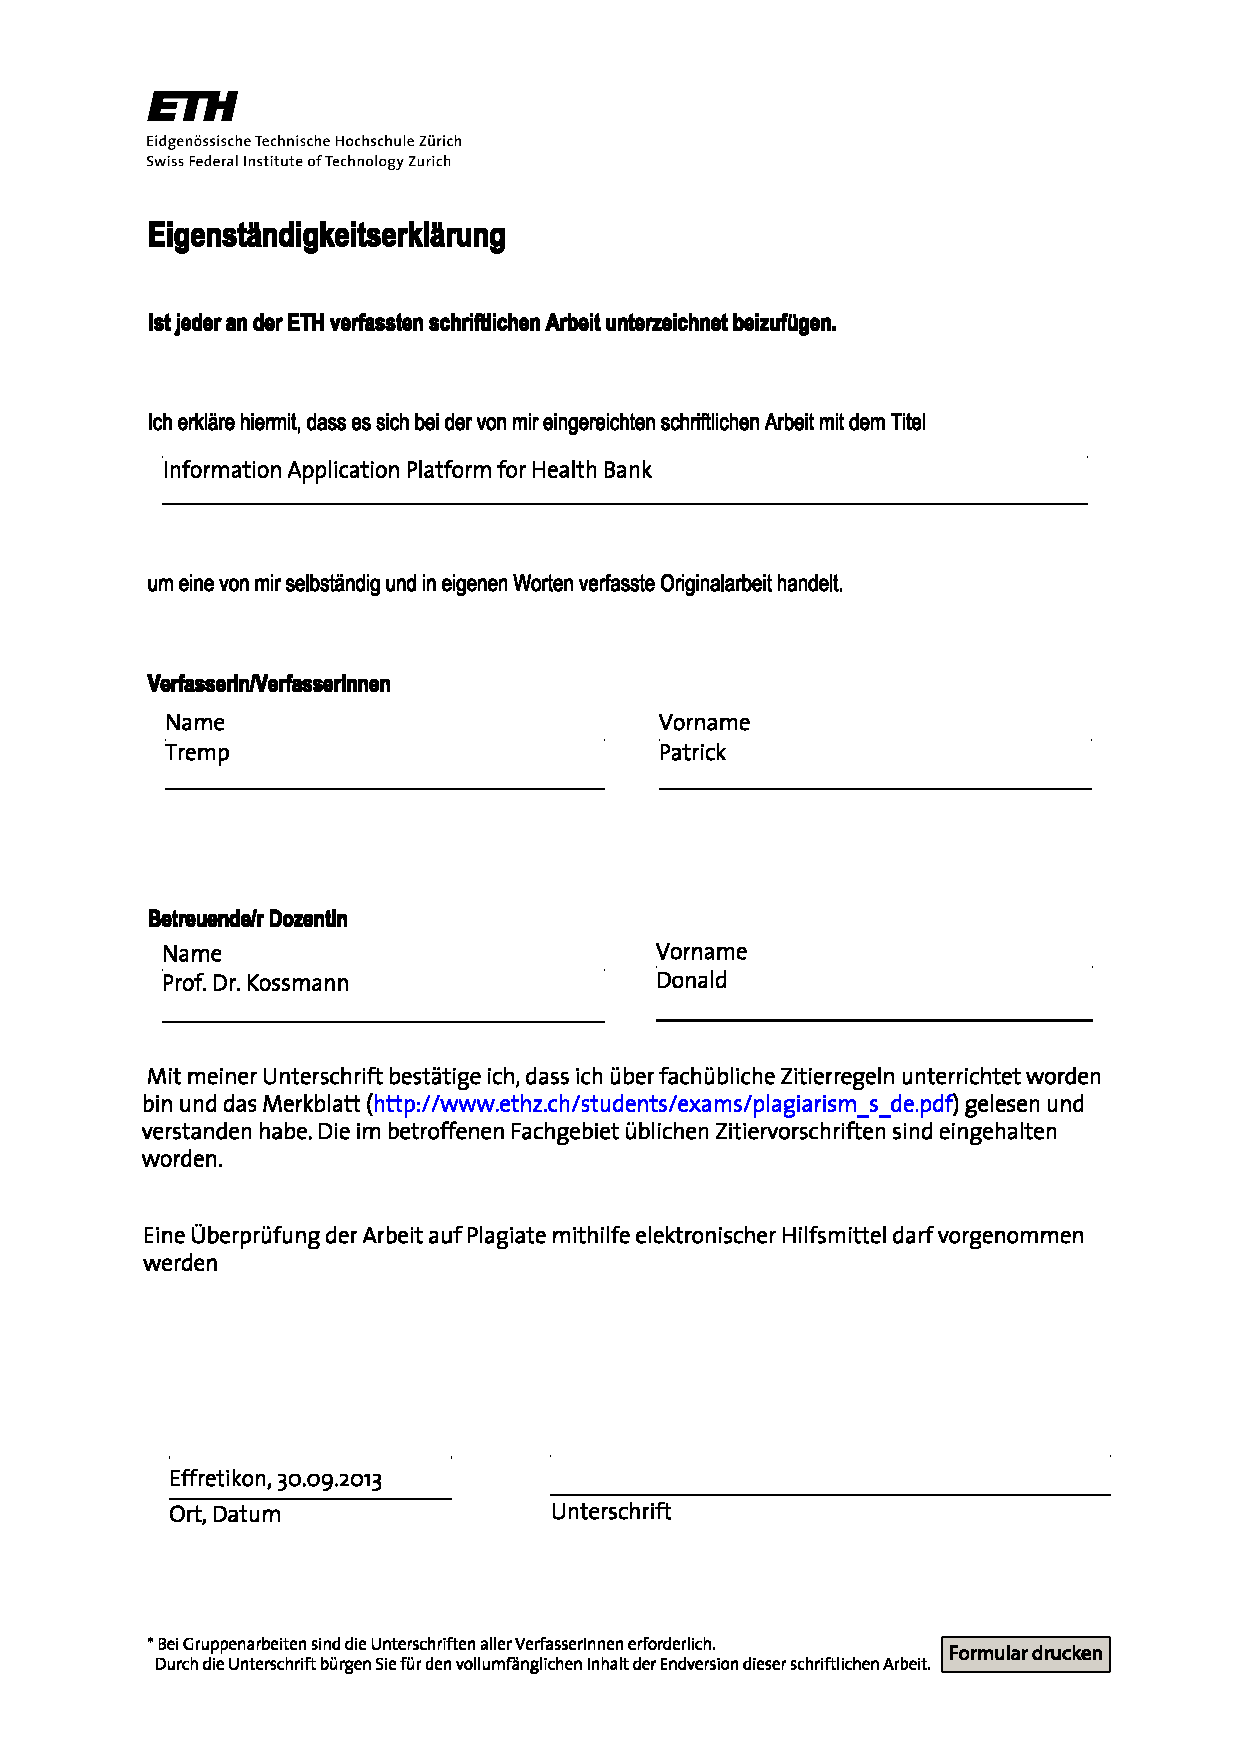
\includepdf[pages=1]{declarationOfOriginality.pdf}
	
\end{document}
